% !TEX TS–program = pdflatexmk
%%%%%%%%%%%%%%%%%%%%%%%%%%%%%%%%%%%%%%%%%%%%%%%%%%%%%%%%%%%
% EPFL report package, main thesis file Goal: provide formatting for theses and
% project reports Template's Author: Mathias Payer <mathias.payer@epfl.ch>
% Thesis's Author : Arnaud Pannatier <arnaud.pannatier@epfl.ch>
%%%%%%%%%%%%%%%%%%%%%%%%%%%%%%%%%%%%%%%%%%%%%%%%%%%%%%%%%%%
\documentclass[a4paper,11pt,twoside=semi,openright]{report}
\usepackage{emptypage}
% Options: MScThesis, BScThesis, MScProject, BScProject
\usepackage[MScThesis]{EPFLreport} \usepackage{xspace}
\usepackage{array}
\usepackage{rotating}
\usepackage{placeins}
\newcommand{\PreserveBackslash}[1]{\let\temp=\\#1\let\\=\temp}
\newcolumntype{C}[1]{>{\PreserveBackslash\centering}p{#1}}
\newcolumntype{R}[1]{>{\PreserveBackslash\raggedleft}p{#1}}
\newcolumntype{L}[1]{>{\PreserveBackslash\raggedright}p{#1}}
\usepackage{arydshln}


\usepackage{booktabs}
\usepackage{caption}
\usepackage{float}
\usepackage{titlesec}
\usepackage{capt-of}
\usepackage{cleveref}


%dashed line
\usepackage{array}
\usepackage{arydshln}
\setlength\dashlinedash{0.2pt}
\setlength\dashlinegap{1.5pt}
\setlength\arrayrulewidth{0.3pt}

%Widows & Orphans & Penalties
\widowpenalty500
\clubpenalty500
\clubpenalty=9996
\exhyphenpenalty=50 %for line-breaking at an explicit hyphen
\brokenpenalty=4991
\predisplaypenalty=10000
\postdisplaypenalty=1549
\displaywidowpenalty=1602
\floatingpenalty = 20000


\title{A Control Plane in Time and Space for Locality-Preserving Blockchains}
\author{Arnaud Pannatier}
\supervisor{Cristina Basescu}
\adviser{Prof. Bryan Ford}
%\coadviser{Second Adviser}
\expert{Prof. Pawel Szalachowski}

\newcommand{\sysname}{FooSystem\xspace}

\begin{document}

\maketitle 

\acknowledgments{I want to give a special thanks to my supervisor Cristina
Basescu for the precious help during the Master Thesis. Sometimes starting in a
new field such as distributed and decentralized systems require a certain level
of abstraction and the advice provided during the weekly meetings allowed me to
have a good understanding of the subject.  \\ I would also like to thank Prof.
Bryan Ford for the supervision of this work. And the external expert, Prof.
Pawel Szalachowski, for his involvement in the corrections. \\ It was a
pleasure for me to have the chance of working on this Master Thesis during the
same time as Bastian Nanchen. The master's thesis can sometimes feel like a
solitary journey, and it was nice to be able to rely on a friend during this
time. \\ I want to thank Marion Bourqui for her support on a daily basis,
especially during the last three weeks of the master's thesis where the work
was the most intense.  }


\makeacks
\let\savecleardoublepage\cleardoublepage
\let\cleardoublepage\clearpage 

\maketoc

\let\cleardoublepage\savecleardoublepage


%%%%%%%%%%%%%%%%%%%%%%%%%%%%%%%%%%%%%%%%%%%%%%
\chapter{Introduction} %%%%%%%%%%%%%%%%%%%%%%%%%%%%%%%%%%%
%%%%%%%%%%%%%%%%%%%%%%%%%%%%%%%%%%%%%%%%%%%%%%

%% Presentation and setting
Distributed ledgers were the trend of the last ten years. You might realize
that when your hairdresser starts to tell you that he plans to put his money
into blockchains or when your little cousin asks to have some Bitcoin
\cite{Nakamoto2009} for Christmas. The research in this field is growing every
year.

However, distributed ledgers still have weaknesses. The purpose of this
work is to propose a solution concerning two well-known weaknesses. The first
one is the time required to confirm a transaction. Indeed, in Bitcoin
\cite{Nakamoto2009}, validating a transaction can take around one hour, because
it takes around ten minutes to validate a block, and it needs around six blocks
to be convinced with a high probability that the ledger won't be forked, and
the transaction invalidated. This might be acceptable for some transactions of great
value. For example, if somebody is buying a car using Bitcoin
\cite{Nakamoto2009}, this person might agree to wait one hour so that its
transaction is validated. However, if somebody wants to use it to buy its daily
coffee, he might be a bit annoyed to wait that long. The other weakness
appears in World War III scenarios. If a third World War occurs, splitting the
World in two, one can expect that the circumstances would cut the communication
between the two sides. This is a problem for standard distributed ledgers as it
is leading to forks that the system cannot resolve at the end of World War III.

This work is part of a larger project called Nyle [\autoref{fig:Nyle}], which
uses the notion of locality to solve these problems. The idea is to replicate
the system along regions of different sizes, from local (e.g., Switzerland,
London) to global.  With this idea, a transaction can be validated in a local
region first, but it is still possible to wait for global validation if needed.
Most of the time, a transaction that was validated locally is validated
globally as well. Still, in some cases, when propagating the information to the
global regions, some transactions might be invalidated as they are in conflict
with others. Therefore one or both won't be accepted to avoid double-spending.
For significant transactions, people might prefer to wait for global
confirmation. Nevertheless, if one wants to buy its daily coffee, local
validation might be enough for the merchant, especially if he already knew the
person. For World War IIIs Scenarios, Nyle offers a solution as well, indeed if
a global partition occurs, the system replicated in smaller regions that are
not split by a partition can continue working flawlessly. 

\begin{figure}[!h] \centering \includegraphics[width=400pt]{figures/Nyle}
    \caption{Sketch of Nyle: The Blockchain is replicated across all regions.}
\label{fig:Nyle}
\end{figure}

%% Main Challenge
Nodes that are spread over the World are maintaining Nyle's distributed ledger.
Clients can ask the nodes to proceed with their transactions or other requests.
Nodes are participating in a different number of regions. A first challenge is
to draw these regions adequately. A second challenge is \textit{churn}: in an
internet-like network with \textit{open-membership} the control plane should be
dynamic, as nodes can join, leaves or move in the system at any moment. This
challenge might not be a problem for classic distributed ledger as Bitcoin
\cite{Nakamoto2009}, as its protocol only takes into account the computational
power that is in the system at a given time. But as Nyle is locality-based,
this might lead to additional challenges, each corresponding to the different
actions possible: joining, leaving and moving.

For joining nodes, consider the case where there were only a few nodes spread
along a vast region, for example, Western Europe, and after a while, a large
number of new nodes want to join there. If region creation is not allowed, this
big region stays the smaller unit of locality, and this might lead to some
problems.  Furthermore, for a region of this size, the probability of a
partition is relatively substantial. One might want that the joining of new
nodes creates additional regions with the size of countries, for example.
Therefore, regions should be able to adapt, depending on node membership. If
nodes leave the system, this might lead to problems as well. Indeed if too many
nodes leave, some regions might not contain any nodes that are maintaining the
system. To avoid this situation, it could be possible to modify the regions
when nodes leave to guarantee that a sufficient number of nodes are in a region
at any time. Moving nodes are creating problems as well with fixed region
assignment. As nodes are mobile, a node can drift apart after a while far away
from his assigned regions. This drifting might take a while, but one can
imagine the situation where many nodes have moved far away from their original
position. In case of a global partition, this can lead to the failure of even
small regions, that is one problem to avoid in Nyle. Therefore the regions
should be adapted with the movement of the nodes. 

%% Related Work Is Insufficient
CRUX \cite{Basescu2014} is the basis of most of this work, which introduces an
algorithm that allows creating regions based on compact graph theory.
\Cref{chap:Background} describes this algorithm in more detail. This work uses
the existing code base for CRUX in Go. A first work on Nyle \cite{Sierro2019}
proposes a first implementation of Nyle building on the top CRUX
\cite{Basescu2014} but focusing directly on how to improve the storage of the
transactions and the tree structure of the regions. This work builds directly
upon the existing work, but is slightly orthogonal, as the Control Plane has
not a direct relation to the replicated blockchain. Sabrina Kall
\cite{Kall2019} has done a second work on Nyle, called
\textit{proof-of-location}. Her work is proposing first, a way of checking the
location of a node efficiently. And second, a method to assert if nodes were
lying about the location where they claimed to be. There is a current work by
Guillaume Michel on the Interplanetary-File System (IPFS) \cite{Michel2019}
that is based on CRUX as well but with the purpose of creating a locality-aware
overlay to speed the system up. However, it is not directly related to
blockchains. \Cref{chap:RelatedWork} describes the rest of the related work.
These works are mostly orthogonal to the current approach: some other solutions
to speed the validation of transaction are Bitcoin \cite{Nakamoto2009}, Byzcoin
\cite{Kogias2016}, Omniledger \cite{Kokoris-Kogias2017}, DFINITY
\cite{Hanke2018}, Monoxide \cite{Wang2019} and Stellar \cite{Lokhava2019}.
However, they don't use the concept of the locality for this purpose. 

%% Description of the Approach
Here is the structure of this work: first, a simple version of the control
plane was designed in \Cref{chap:Design}, which splits the time into epochs and
takes as an assumption that the system remains fixed during one epoch. This
work proposes and discusses a protocol, and gives his threat analysis.  Based
on its implementation and performance analysis, some drawbacks are put into
light. Then a series of strawman models try to correct some of these drawbacks
and are analyzed as well in \Cref{chap:Improvements}. The first one is called
"Locarno Treaties" and try to keep the system coherent from one epoch to the
next. The next one is called "Fog of the war", and try to reduce the need for
communication between nodes. The last and the most complex Strawman considers
the interactions of the nodes as a space-time graph and try to build upon the
existing patterns that appear in these graphs to propose a different notion of
distance. 

%% Thesis Statement
This work proposes \textbf{A Control Plane in Time and Space for
Locality-Preserving Blockchains}. This control plane for Nyle is needed to
ensure to have a \textit{open-membership} and to solve the problems of World
War III scenarios and to allow regional validations. The series of strawman
models improving the simple control plane leads to the use of Space-Time graphs
that allowed to improve the existing design. 

%%%%%%%%%%%%%%%%%%%%%%%%%%%%%%%%%%%%%%%%%%%%%%
\chapter{Related Work} \label{chap:RelatedWork} %%%%%%%%%%%%%%%%%%%%%
%%%%%%%%%%%%%%%%%%%%%%%%%%%%%%%%%%%%%%%%%%%%%%

This work builds upon several other works in the domains of blockchain and
locality. Nyle proposes a decentralized cryptocurrency using different
strategies than Bitcoin \cite{Nakamoto2009}, Byzcoin \cite{Kogias2016},
Omniledger \cite{Kokoris-Kogias2017}, DFINITY \cite{Hanke2018}, Monoxide
\cite{Wang2019} and Stellar \cite{Lokhava2019}. But it uses them as a source of
inspiration and shares some aspects with these general cryptocurrencies. It is
somehow orthogonal to them because it can use any of these cryptocurrencies as
an underlying system and enhance them using the idea of the locality to provide
them with some partition-resistance and regional validation. 

These works are the direct source of inspiration for some key concepts of this
work. DFINITY \cite{ Hanke2018} directly inspires the Sybil-resistant scheme
used in the registration system, using \textit{endorsement} in the general way,
which can be in practice replaced by any Sybil-resistance scheme like
Proof-of-Work \cite{Nakamoto2009}, Proof-of-Stake \cite{wood2014ethereum}, or
even Proof-of-Personhood \cite{Borge2017}. In particular, this work tries to
solve some drawbacks of traditional cryptocurrencies like Bitcoin
\cite{Nakamoto2009}, solving the problem of the waiting time for transaction
validation by using regional validation and making it resistant to WWIII
scenarios. Byzcoin \cite{Kogias2016} and Omniledger \cite{Kokoris-Kogias2017}
give another interesting solution to accelerate the validation, but their
results are orthogonal to this research. Stellar's solution for
\textit{open-membership} \cite{Lokhava2019} is based on a quorum, allowing each
node to trust a subset of other nodes of its choice. It is an elegant solution
and permits to validate transactions fast and securely. A certain complexity
seems to be added both in the theoretical and practice part. This justifies why
a similar approach was not followed. However, the idea to allow nodes to have a
different view of the system is at the core of one of the improvements of this
work, described in \autoref{sec:Fog-of-the-war}.

Omniledger \cite{Kokoris-Kogias2017} and Monoxide \cite{Wang2019} use sharding
to increase performance. Sharding, which splits the system in a random
committee that allows the fastest processing of the transaction. Sharding is
orthogonal to the replication process used in this work. As even if the system
is split into different parts, first, it is not done randomly but based on the
locality. Furthermore, the system is replicated in all regions. However,
cryptocurrencies using shards can still be used as an underlying system of
Nyle, enhancing the performance of the partition-resistant blockchain system
created by this means.

This work is directly related to the locality-preserving algorithms developed
in CRUX \cite{Basescu2014} and compact-graph algorithms \cite{Thorup2005},
which are described in detail in \Cref{chap:Background}. There is a class of
algorithms that uses the idea of locality differently. For example, Geo-DNS
\cite{Katz-bassett2006} or IP Anycast \cite{Abley2006} use the locality to
shorten the path for the packets, connecting the servers via the closest path.
Replication is often used to guarantee the integrity of the stored information
\cite{Mokadem2015}. In CRUX \cite{Basescu2014} and Nyle regional replication of
the system is used to create partition-resistance, and in Nyle, it can be used
to allow region validation.

Some classic consensus protocols as PAXOS \cite{Lamport2000}, PBFT
\cite{Castro1999} were used as an inspiration to the protocol. In practice, and
for efficiency, this work uses BlsCoSi \cite{Boneh2018} that is much more
efficient, because it makes smart use of trees for communication. BlsCoSi
\cite{Boneh2018} is still prone to some failures in case of successive
view-changes, it could be improved using a different protocol such as HotStuff
\cite{Yin2018} which solves the problem of view change using a third round of
communication. 

This work uses a distributed public algorithm for the source of randomness like
Randhound \cite{Syta2016}. Each node uses this source to draw a random level.
The way it is used is described in detail in the next section. 


%%%%%%%%%%%%%%%%%%%%%%%%%%%%%%%%%%%%%%%%%%%%%%
\chapter{Background} \label{chap:Background} %%%%%%%%%%%%%%%%%%%%%%
%%%%%%%%%%%%%%%%%%%%%%%%%%%%%%%%%%%%%%%%%%%%%%

This Master Thesis is part of a larger project that concerns
locality-preserving systems. In particular, it builds upon CRUX
\cite{Basescu2014} and is part of Nyle. This section describes two different
projects. 

\section{CRUX - Fast and Resilient Datastore with Automated Locality}
\subsection{Description} CRUX \cite{Basescu2014} introduces a smart way of
dealing with partitions in decentralized systems. Partitions occur in
decentralized systems, but one can try to find a solution to reduce their
effects on the global system. For example, if a partition occurs, there are no
reasons that nodes that are functioning on the same side of the partition
should stop working because of the partition. 

The general idea is that a system can be replicated at different scales, from
local (big cities, small countries) to global. The replication means that a
separate instance of the system is created in all regions.  This ensures the
additional property that each replicated system continues to work correctly if
no partition splits it. If a global partition occurs, then the global region
might not work, but all the replicated systems in local regions continue
working. This is a direct solution to the previously mentioned problem: nodes
working on the same of the partition continue to work. The force of CRUX is
that it provides a locality property  \cite{Basescu2014}. For \textit{any two
nodes} in the system, it is guaranteed that they participate within a region
with a radius that is equal to a small multiple of their \textit{Round Trip
Time} (RTT).

This solution comes with an overhead, as the system should be replicated in all
the regions. However, there are ways to reduce these overhead costs so that
they remain reasonable and that resistance to partition is maintained. CRUX
algorithm for regions creation \cite{Basescu2014} presented below ensures that
the proper number of regions is created in a manner that the number of regions
created induces a reasonable overhead and that the partition resistance stays
efficient. If CRUX \cite{Basescu2014} is used for a specific system, overhead
can be even more reduced: as the systems are replicated in every region, most
of the data is replicated as well. So one might dig inside the specification of
one system and manages not to store twice the same data. But this goes beyond
the goal of CRUX \cite{Basescu2014}, which wants to be the more general
possible. 

Indeed, the force of CRUX \cite{Basescu2014} is that it applies to any
distributed system, as no particular hypothesis on the system is made. It only
starts from a straightforward idea: one system can be replicated at a smaller
scale to ensure some partition resistance. 

A note should be made about the CAP-theorem, which states that no system can be
consistent, available and partition-resistant at the same time. It seems that
this solution is adding partition tolerance to an available and consistent
system, thus leading to the violation of the theorem. But it is not precisely
the case, as the enhanced system only ensures that nodes can still work in some
regions that are not affected by the partition. The regions split by a
partition are not working anymore. Even if the system can still work on the
same side of a partition, it's not partition resistant as a whole.

\subsection{Common Tools} \label{sec:common-tools} This section describes how
to create regions that are used to replicate the system. These regions are used
by Nyle as well. These regions are called \textit{Available Responsive Areas}
(ARA), in each region, a copy of the replicated system is deployed. Each node,
starting at level 0, participates first at a lottery. Then each node goes to
the next level with a given probability $P$. This procedure is repeated at
every level and is stopped when no nodes are promoted to the next level. This
first empty level is called $K$. Then each node can compute two quantities that
are necessary to create \textit{ARAs}: their bunch and their cluster. 
 
\begin{table*}[h!] \centering
\begin{tabular}{@{}ccccc@{}}\toprule
\textbf{System} & \textbf{Level $\#1$} & \textbf{Level $\#2$} & \textbf{Level $\#3$} & \textbf{Level $\#4$} \\ \midrule
100 & 90 & 9 & 1 & 0 \\ \hdashline
200 & 180 & 18 & 2 & 0\\ \hdashline
 500 & 450 & 45 & 5 & 0\\ \hdashline
 1000 & 900 & 90 & 9 & 1\\ %\hdashline
\midrule
$N, k=2$ & $N(1-p)$ & $Np(1-p)$ & $Np^2$ & $0$ \\ \hdashline
$N, k=3$ & $N(1-p)$ & $Np(1-p)$ & $Np^2(1-p)$ & $Np^3$ \\ %\hdashline
\midrule
\bottomrule
\end{tabular}
\caption{Example of lottery with $P = 0.1$ where $k= 3$ for $N= 100,200,500$
and $4$ for $N = 1000$. Columns represents the number of nodes and the row the levels. }
\label{example-lottery}
\end{table*}
 
\begin{figure}[!h] 
\centering
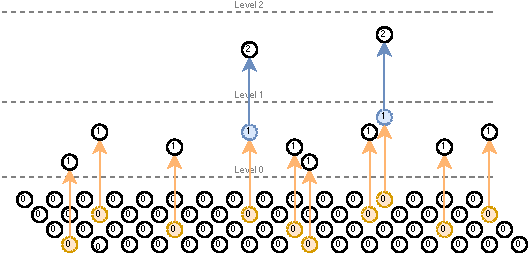
\includegraphics[width=400pt]{figures/Lottery-Standard}
\caption{Sketch of the Lottery process, nodes goes from one level to the next
  with probability $P$} \label{fig:ClusterBunch-Bunch}
\end{figure}

\paragraph{Bunch} A node can compute its bunch in the following manner. It
looks at every other node by order of distances in ascending order and
includes it in its bunch if its level is not smaller than any level it encountered
so far, including its level [\autoref{fig:ClusterBunch-Bunch}]. 

\begin{figure}[!h] 
\centering
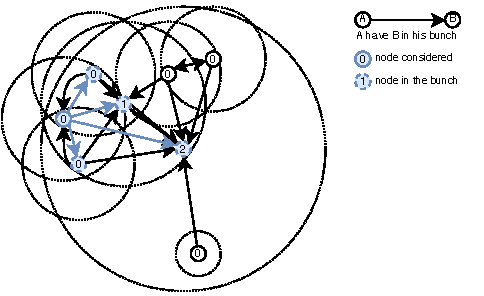
\includegraphics[width=350pt]{figures/ClusterBunch-Bunch}
\caption{The bunch of the  level-0 blue node with solid border is depicted in
    blue. The cluster of the higher level node covers the whole system.}
    \label{fig:ClusterBunch-Bunch}
\end{figure}

\paragraph{Cluster} A cluster is a complementary concept. The cluster of node
$A$ is defined as the set of other nodes that have $A$ in their bunch
[\autoref{fig:ClusterBunch-Cluster}]. 

\begin{figure}[!h] 
\centering
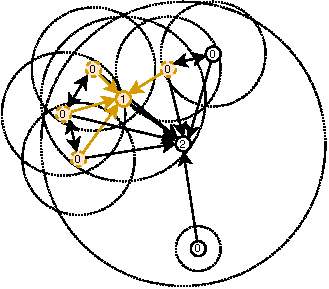
\includegraphics[width=350pt]{figures/ClusterBunch-Cluster}
\caption{The cluster of the level-1 orange node is depicted in orange. The
    cluster of the higher level node covers the whole system.}
  \label{fig:ClusterBunch-Cluster}
\end{figure}

\begin{figure}[!h] 
\centering
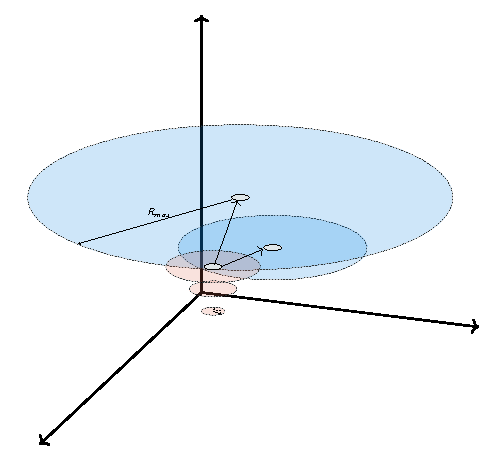
\includegraphics[width=350pt]{figures/regions/ellipsis}
\caption{ A node (red) participates in two kinds of regions. The ones it
    creates with a radius from $R_{min}$ to one that is covering its cluster
    (orange). And some regions created by the nodes in its cluster, which are
    covering him (blue).} \label{fig:RegionCreation}
\end{figure}

The smallest region radius $R_{min}$ is defined for the whole system. Each node
constructs $ARAs$ around itself, starting at $R_{min}$ and doubling the
radius at each time. It stops at the first $ARA$ that is covering its entire
cluster [\autoref{fig:RegionCreation}]. 

By the lottery, most nodes are level-zero nodes. Therefore, their clusters are
supposed to be small, conducting to the creation of a small number of $ARA$s.
The small number of nodes that are at level $K-1$ have every other node
in their cluster by construction. This means that there is  at least one
$ARA$ that covers the whole system. 

\section{Nyle - A Locality-Preserving Blockchain}

Nyle is a cryptocurrency that uses locality to answer some classical problems
of blockchains. Two central problems are addressed: WWIII scenarios and approval
time for a transaction.
 
\paragraph{WWIII Scenarios} \label{WWIII} In case of a WWIII, we can expect to
have at least a long-lasting partition that split the system in two. This
is a problem for classical cryptocurrencies like Bitcoin \cite{Nakamoto2009}
because for a block to be approved, the users are supposed to wait to have a
global consensus. This consensus will not be reached with a long-lasting
partition and therefore, it creates problems for classical cryptocurrencies.
Nyle solves this issue by design using locality.

\paragraph{Approval Time for a Transaction} \label{approve_time} Another issue
with waiting global consensus is that it usually takes a long time. If a
customer wants to use a cryptocurrency in daily life, the nodes should be able
to validate (at least partially) transactions relatively fast. The solution
provided by Nyle uses locality again: a transaction can be validated at
different geographical levels, and it is up to the customer to wait for a
local, or global validation for a transaction. For small transactions, e.g.,
for buying a coffee, the customer might agree only to have local validation.
For more significant transactions, he might want to wait a bit longer to have
global validation.

\subsection{Description}

Nyle uses \textit{ARAs} as the representation of one region. In each of these
regions, there is a copy of the same system; in the case of Nyle, the
system is a blockchain. So each region has its blockchain and validates
all the transactions between the nodes that are included in it. Some nodes can
be contained in different regions, and they send their transactions to all
the regions they are part of. As all nodes participate in the global region by
design, this ensures that a transaction is eventually seen by all nodes.

The big difference between CRUX \cite{Basescu2014} and Nyle is that the purpose
of CRUX \cite{Basescu2014} is to work in environments where machines are
relatively "stable" which means that they are not supposed to churn,
where the machines are not supposed to move or to join, and more importantly,
where nodes are not malicious. This is not the case for Nyle: if we have a
cryptocurrency, we can expect to have deficient, malicious and moving nodes.
This adds some difficulties that are managed by the protocol.

Each region has its blockchain. In Nyle, the choice for the blockchain is
chosen between ByzCoin \cite{Kogias2016} or Omniledger
\cite{Kokoris-Kogias2017}, but it can be generalized to any blockchain.

\subsection{What is already implemented for Nyle} \paragraph{CRUX algorithm for
region creation} We already have an algorithm for drawing regions
\cite{Basescu2014}.

\paragraph{Block storage on node} As each node participates in different
regions (from very local to worldwide), it needs to store the blockchain
for all of these regions. We have a method that reduces the redundancy, by only
storing the hash of a block instead of the full block at each level
\cite{Sierro2019}. 

\paragraph{Proof-of-Location} We already have a protocol for controlling the
distance from a new node to the rest of the nodes, and that assures no one
cheats by giving false distances \cite{Kall2019}. 

\subsection{Purpose of This Project: Motivation for a Control Plane}

CRUX \cite{Basescu2014} proposes a system that is working in a stable system
(with low-churn) and where nodes do not move too much. This situation
corresponds to some systems like a wide-area database. It is not
the case of a cryptocurrency. For this kind of system, one can expect to have
at least some churn, some moving nodes and some joining nodes. If the
system has a precise protocol for dealing with nodes entering, leaving and
moving in the system, then the problem of the evolution of the system is
solved. Indeed the churn phenomenon can be described as some nodes leaving the
system and optionally reentering later. 

CRUX \cite{Basescu2014} can still envisage the use of a control plane, and it
considers it as future work. As even if CRUX  \cite{Basescu2014} does not have
high churn, the \textit{RTT} between nodes can still vary. 

Therefore the purpose of the control plane is to manage the regions in order to
follow the evolution of the nodes in the system. Once that problem is solved,
the blockchain can be replicated in the evolving region and the strategy is the
same as in CRUX \cite{Basescu2014}. This project introduces a control plane,
that is in charge of the evolution of the nodes. In particular, it is in charge
of dealing with nodes joining, leaving and moving. The blockchains are
replicated in all the regions, but the control plane is global. 

%%%%%%%%%%%%%%%%%%%%%%%%%%%%%%%%%%%%%%%%%%%%%%
\chapter{Design} \label{chap:Design} %%%%%%%%%%%%%%%%%%%%%%%%%%%
%%%%%%%%%%%%%%%%%%%%%%%%%%%%%%%%%%%%%%%%%%%%%%

This part describes the design of the Control Plane, which has the mission to
solve the problem of node insertion, deletion and movement inside the system. A
first version of the control plane is designed, and then it is improved by a
series of Strawman models.

\section{Problem definition}
\subsection{Hypotheses}
Three hypotheses are made on the network. First, it assumes an Internet-like
network with one-to-one communication. Each node can contact any other nodes.
This hypothesis is required as nodes need to communicate for the different
consensus.  Second nodes need to have synchronised clocks, and the protocol
requires this as it assumes that they are two successive periods, one for the
registration and one for executing the system, and nodes should know when they
are supposed to start and to register.  The third hypothesis is made on the
geometry of the network. It states that for small pings (under 100ms), the
round-trip-time is correlated with the distance between two nodes. This is the
case for the Internet network \cite{Seibert2014}. This is required as the
locality component use that hypotheses to estimate distances with pings. On
this result, we build the locality properties of the system. 

\subsection{Threat Model}
Attacks on the system can be made internally from malicious nodes or
externally by delaying the interaction between nodes or intercepting and
forging messages. We give the precise portion of malicious nodes that
this protocol can handle. In this threat model, malicious nodes are regular
nodes that decide to act against the system. In particular, malicious nodes
have only access to limited computational power, and they cannot break the
cryptographic primitives. 

\section{General Presentation}

The Control Plane is composed of five different components
[\autoref{fig:modules}], each necessary to address different parts of the
problem.  It needs a membership component, to define which nodes are in the
system at any time. It needs a distance oracle which gives the distance between
two nodes in the system. Then it needs a region management component, which
creates and alter the regions based on the membership and the locality.  The
time is split into epochs, and a component is in charge of dealing with that
aspect. And finally, the control plane is in charge of answering some requests
linked to the location and presence of the nodes in the system. Each component
is described in detail below. 

\begin{figure}[!h]
\centering
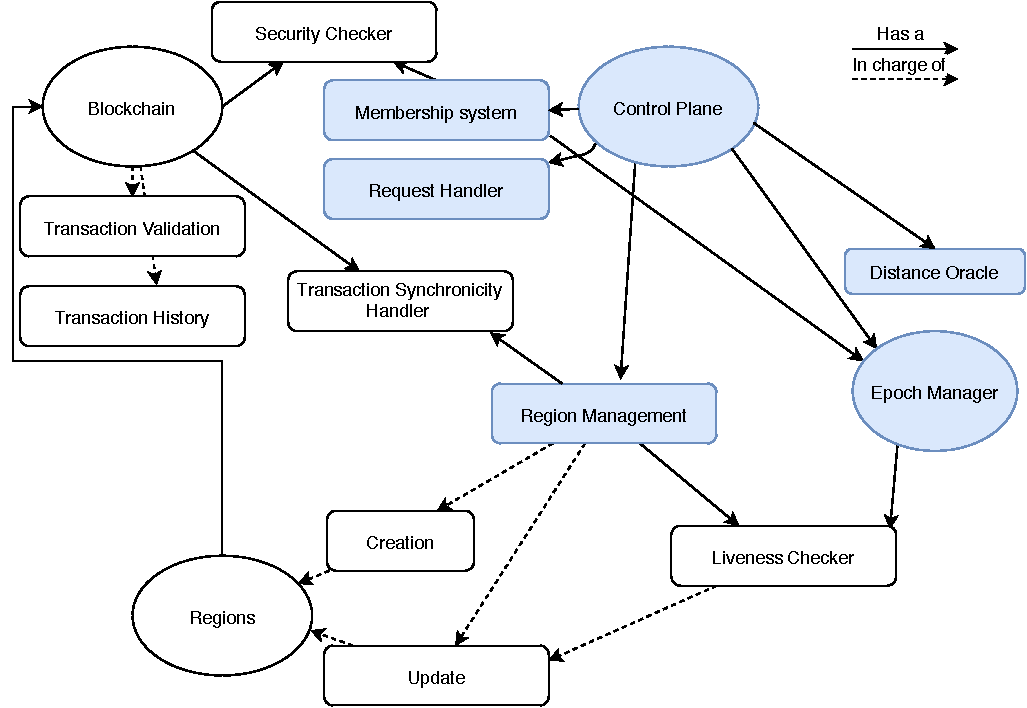
\includegraphics[width=400pt]{figures/Nyle_components}
\caption{List of modules of Nyle. This works concerns the components in blue.}
\label{fig:modules}
\end{figure}

\subsection{Membership Component}

At each epoch, a list of all participants for the current epoch is created and
it is signed by the participants of the previous epoch. It is based on
registration, which is made during the previous epoch. Registration use
\textit{endorsement} (for example solution to a proof-of-work problem). This
system is global. Nodes can ask the participants of the system to know the
identity of other nodes. For a new contract to be validated, it should be
signed by the majority of the nodes of the previous epoch.

\subsection{Distance Oracle}

The role of the locality component is to give all pairwise distances between
nodes of the system. We assume it already exists (distance oracle), or that
nodes can compute it. In this protocol, the metric that is used as a distance
is the latency. Therefore all pairwise-latencies are computed between each node
and every node agrees on them via consensus.

We also assume the existence of a control function that is able to assert the
validity of the distances based on the latencies. 
 
\subsection{Region Component} This component is used to create and update
regions. This part is based on CRUX. At each epoch, CRUX is run based on
the new registration, and regions are created.
 
\subsection{Epoch Component} The epoch manager is linked to the membership
system (we allow to change membership at the beginning of one epoch). New nodes
can register during one epoch and join for the next. If nodes have moved, the
Region component change or maintain their assignment at the beginning of one
epoch. If nodes have crashed, they won't be able to join for the next epoch and
will, therefore, leave the system.

Epochs happen at a defined rhythm, e.g. one day. This frequency can be
shortened to ensure that nodes, wanting to join, do not wait too long, or made
longer if one wants regions not to be redrawn too frequently. 

\subsection{Request Handler} The control plane is responsible for handling
requests as it is aware of the nodes location and region assignment. It is
in charge of answering the request for nodes assignment and nodes location. 

\begin{figure}[!h] 
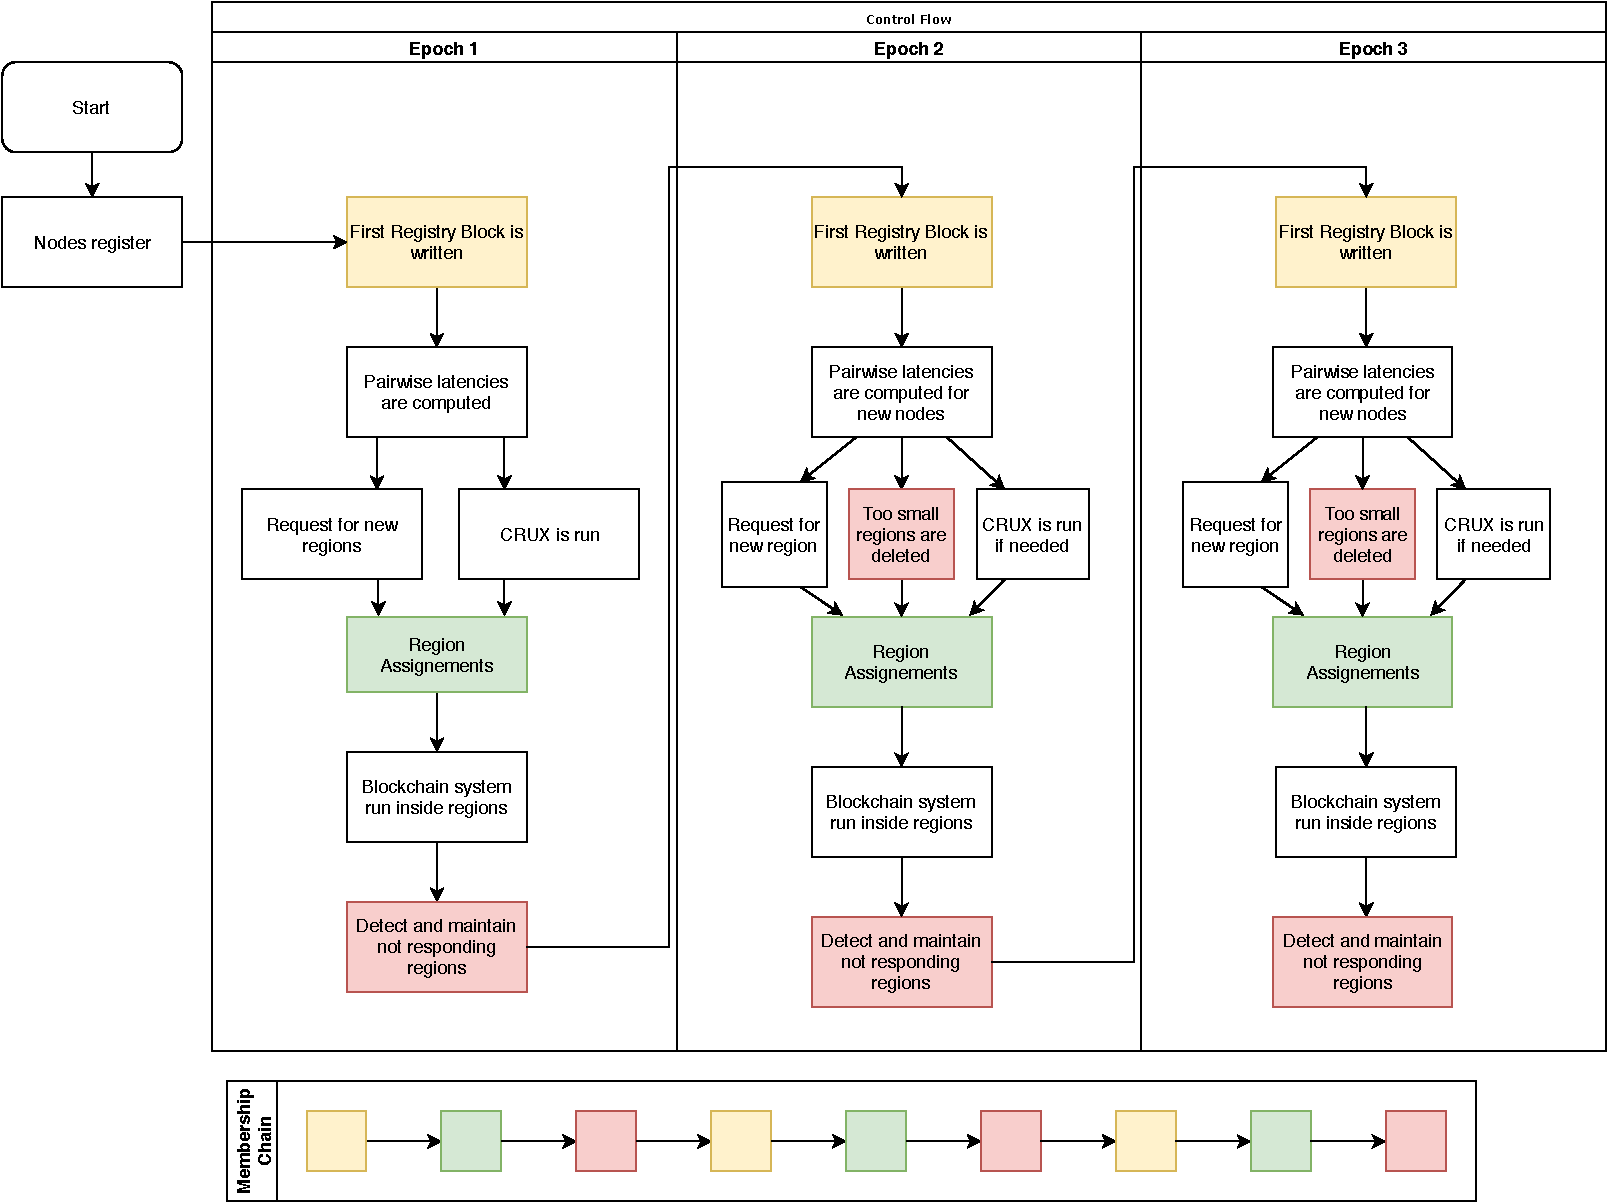
\includegraphics[width=450pt]{figures/Nyle_controlflow}
\caption{General Control Flow of Nyle. }
\label{fig:controlflow}
\end{figure}

\section{Simple Control plane} This version presents the first version of the
Control Plane. In which most of the work is done on the membership component.
At each epoch, nodes can join if they manage to get approval from the members
of the previous epoch. The distance oracle requires many resources: every
node measures pings to every other nodes and consensus is made on that
information. The region component in this model is simple: based on the
registration, and the pings, CRUX is run at each epoch, redrawing the map of
the entire system. 

\subsection{Membership Protocol}

\begin{sidewaysfigure}[!h]
\centering
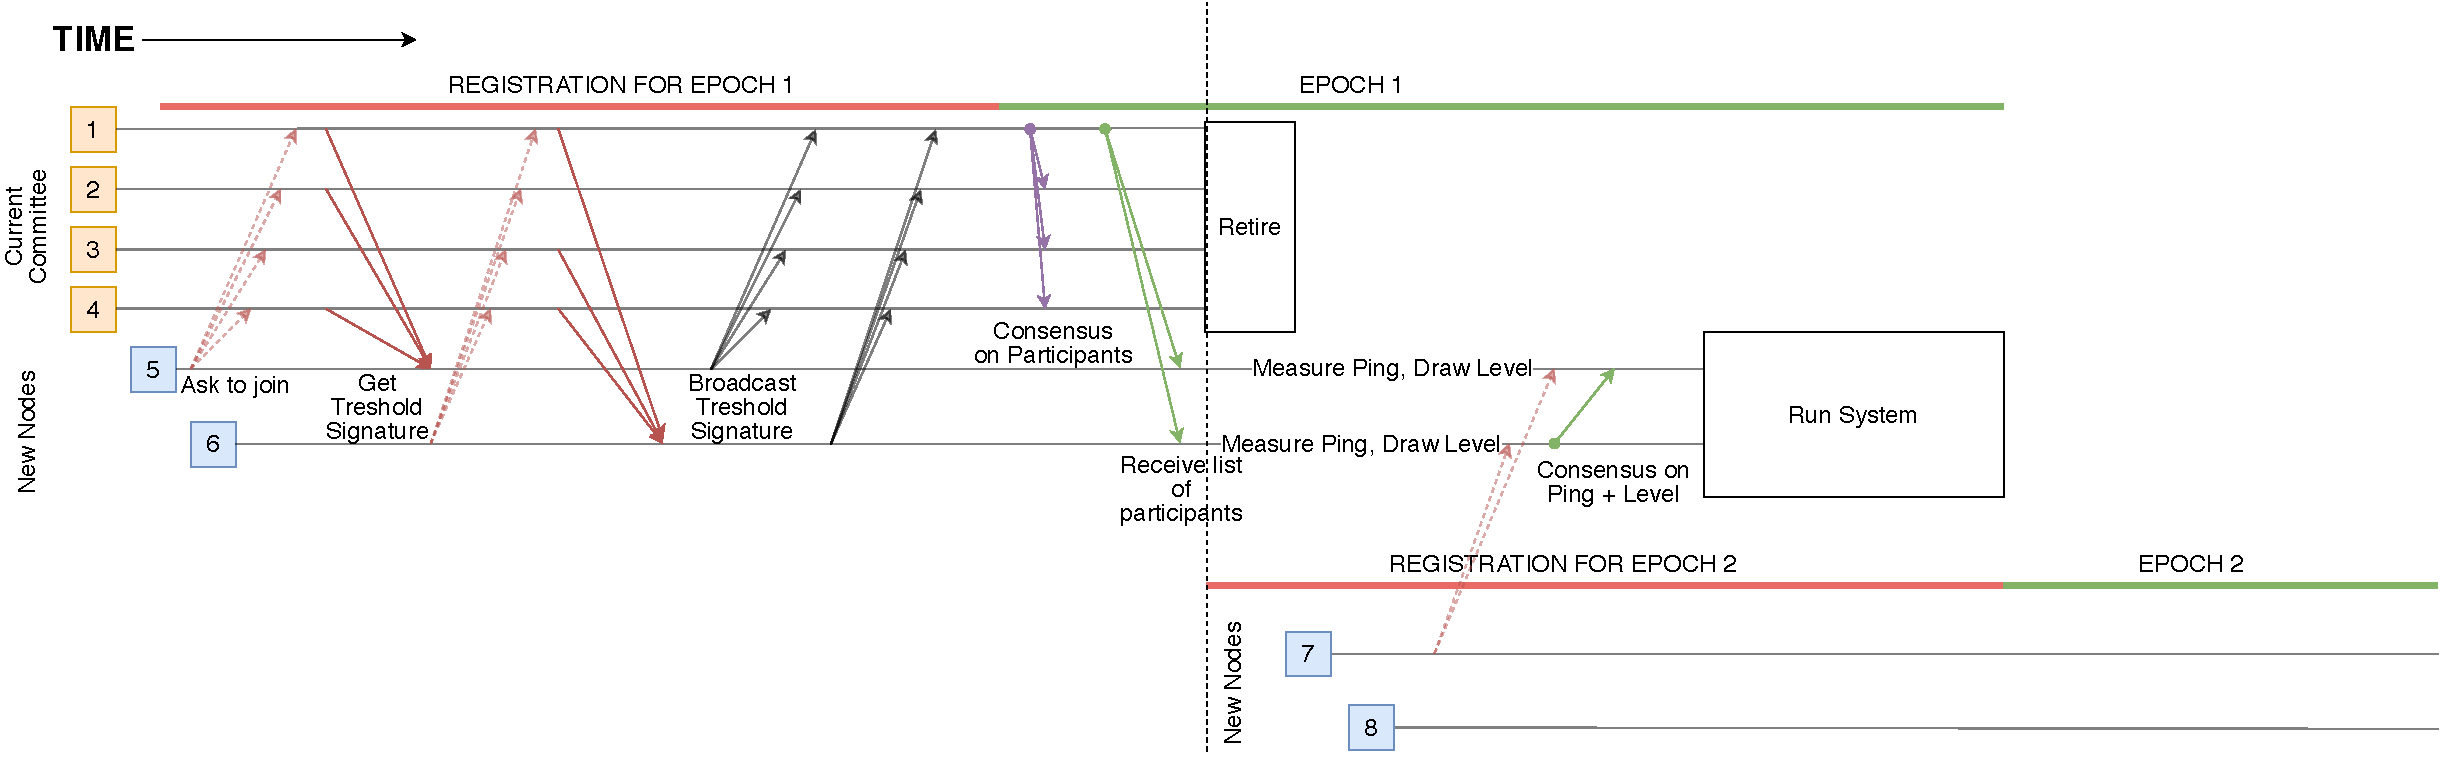
\includegraphics[width=700pt]{figures/Registrationprotocol}
\caption{Sketch of the Protocol.}
\label{fig:registrationprotocol}
\end{sidewaysfigure}

This section describes the membership protocol
[\autoref{fig:registrationprotocol}].  The system goes through some cycles
(called an epoch) of two different phases: the registration period and the live
period. The first period is there to manage the participants of the current
epoch, and the underlying system (e.g., a cruxified-blockchain) is run during
the live period. Assume that each node has a synchronised wall-clock which
gives the time of the different periods.

The authority that decides which node participates in the next epochs is
the participants of the current epoch, which are called the \textit{admission
committee}. Assume that a set of genesis participants, which are the first
 \textit{admission committee}, exists.

\paragraph{Registration Period.}
If a node wants to register for the next epoch, it has to send the following
information to the admission committee: a \textit{name}, a \textit{public key},
and an \textit{endorsement} (e.g., solution to a proof-of-work problem) and ask
for a \textit{threshold-signature}. 

If the new node manages to get back a threshold-signature from the admission
committee, it has to broadcast it again to the admission committee during the
same registration period. The current committee then acknowledges that it
is a participant for the next epoch. This is necessary as nodes in the
committee might not necessarily know if the admission they signed managed to
reach the threshold. The admission committee aggregates the
threshold-signatures for all the participants of the next epoch. At the end of
the registration period, the admission committee reaches a consensus on the
new participants, by threshold-signing the list of the members.  

\paragraph{Live Period.}
At the beginning of the live period, one member of the admission committee
sends the threshold-signed contract that lists the participants to the current
members. If one of the participants did not receive the list, it could ask any
member of the admission committee to have it. After that propagation, the
admission committee can retire, and the members of the current epoch become the
new admission committee. Then members of the new epoch compute the distances
between each other. Participants will as well draw a level from unpredictable,
bias-resistant public randomness source. They reach then consensus on those
ping-distances and levels by threshold-signing them and broadcast them. At this
point, each member of the new epoch has the same view of the system as they
know the participants, the latencies between each one of them and their levels.
Therefore these participants are capable of running the system in a
deterministic manner.

Following the election of the new admission committee at the beginning of the
live-epoch, the registration period for the next epoch can begin, as the
authority that accepts admission is running. Registration period and live
period can, therefore, be superposed [\autoref{fig:registrationprotocol}], which
permits to have a system running at every time. 

\subsection{Threshold-Signing Registration}
To be admitted in the next phase, a node uses the BlsCoSi protocol
\cite{Boneh2018}. It generates a tree with him as the root and the admission
committee as nodes in the tree. Each node of the admission committee has the
choice of signing or rejecting the admission request. The threshold is set at
the majority. So if a node manages to get a majority of signatures, then it is
accepted in the system. A node from the admission committee is supposed to
accept the query if it has not already seen the node, and if the
\textit{endorsement} is convincing and was made with the public-key associated.
This ensures that a node cannot steal the endorsement of another for
registration.  

\subsection{Committee Consensus}
Committee consensus is used at two different times. First, at the end of the
registration period. Consensus should be reached by the admission committee to
agree on the participants of the next epoch. A random member of the admission
committee is selected to run the consensus protocol. It sends the list of
members it has aggregated during the registration period, and try to get a
threshold signature on it from the other member of the admission committee.
Members of the admission committee are supposed to sign the list if they
aggregated the same list of members for the next epoch.

If one member does not achieve consensus, another can be selected to
run the consensus. A communication round can be added between two consensus
phases so that every member of the admission committee broadcast its list
of members with valid proofs.

The same idea is used at the beginning of the live epoch to reach consensus on
the list of pings between every member of the system and on the levels on all
nodes in the system.

\subsection{Public distributed source of randomness}
A distributed public source of randomness is used to draw the levels for the
region creation algorithm. This can be targeted by adversaries trying to get a
specific level which can unbalance the system, as described in
\autoref{app:unbalanced-levels}. To be sure that this source is not targeted,
it is based on the information created during the consensus on the participants
just before drawing the regions. 

\FloatBarrier \section{Details}
\subsection{Advantages}
This simple version of the control plane is solving the problem of node
insertion, churn and nodes movement in the system. A comparison is made
with a fixed version only using CRUX for region management but without a
control plane. Then the system begins with a fixed number of nodes and creates
regions based on CRUX, then it is replicated inside all regions, with
no update possible.

\subsubsection{Nodes Insertion}
The version without a control plane cannot add nodes to the system. Indeed a
fixed number of nodes is required to create the regions. With this control
plane, node insertion is possible at the beginning of every epoch
[\autoref{fig:insertion-comparision}].

\begin{figure}[!h] 
\centering
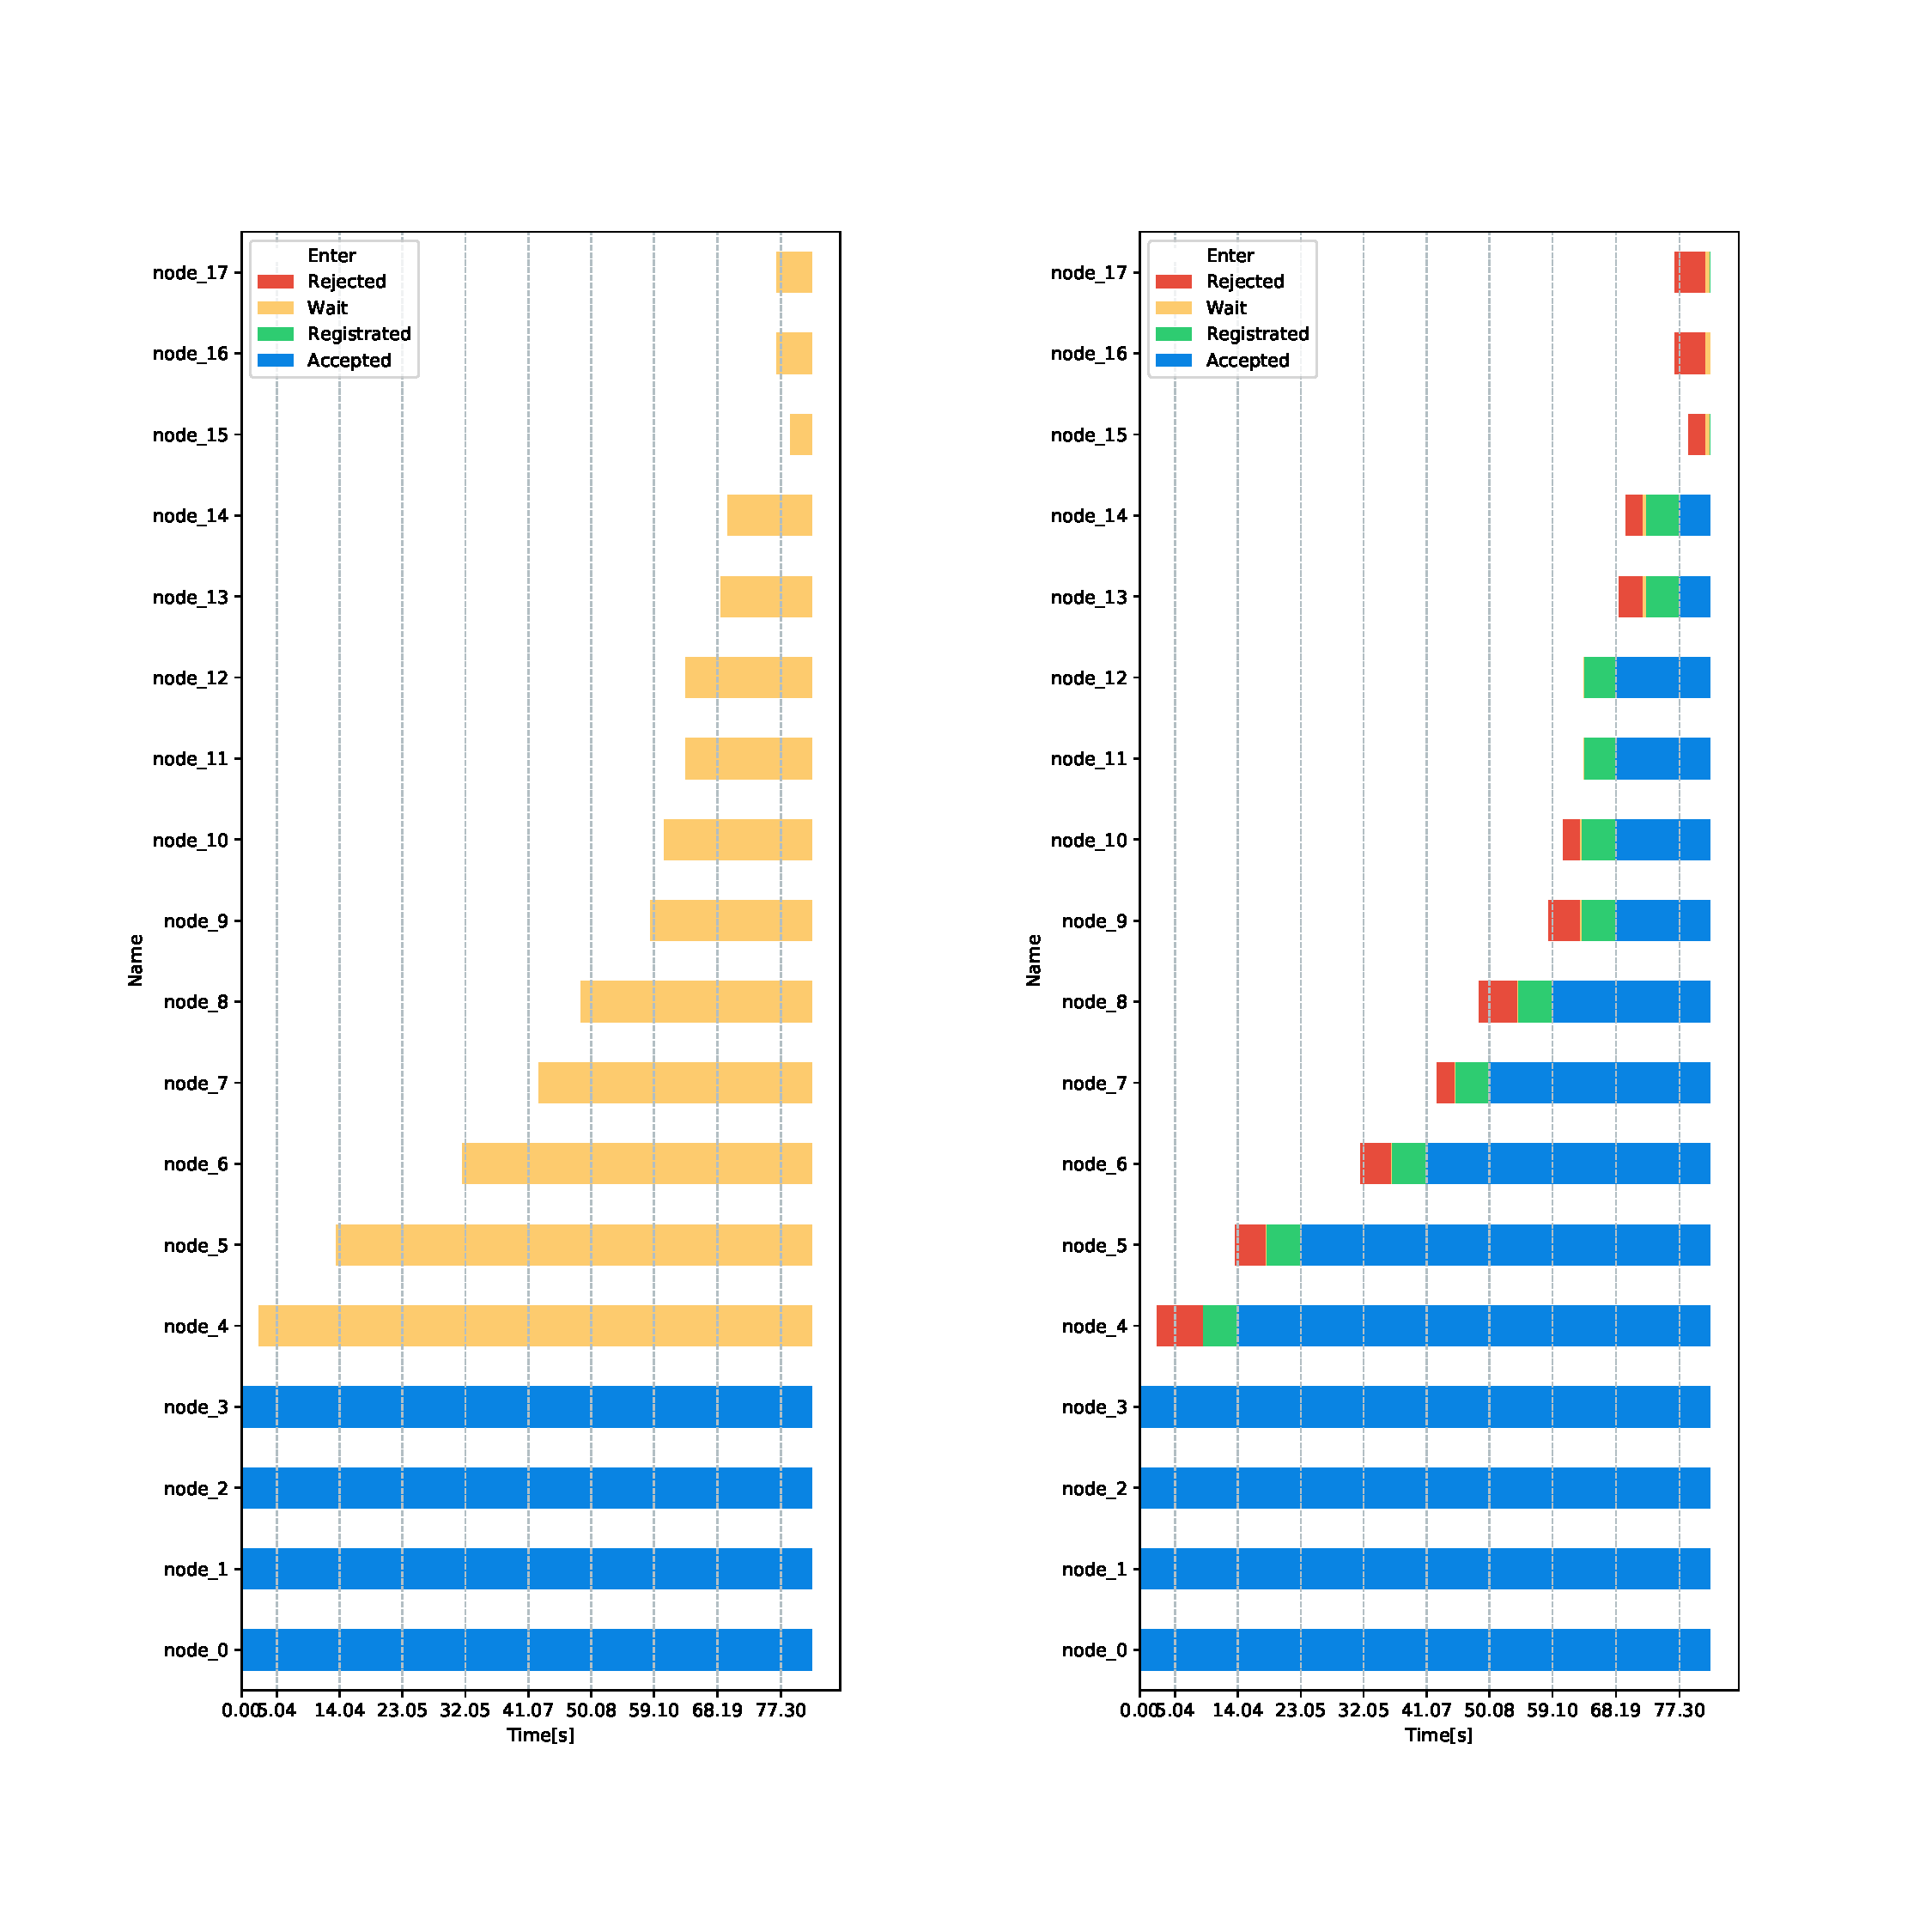
\includegraphics[width=450pt]{figures/JoinSubplots}
\caption{The simple control plane (right) allows nodes to join the system. The
    left plot represents the case with a fixed control plane where nodes cannot
    join. The ticks are placed at the start of epochs. Some registrations are
    refused for the next epoch as they started too late. In these tests, nodes
    that are not passing the registration wait a bit to ask for a new
    registration. The waiting time is really short, as the registration are
    possible at any time due to the superposition of the live period and the
    registration period. }
 \label{fig:insertion-comparision}
\end{figure}

\subsubsection{Churn Resistance}
Nodes can churn. If the system is not supposed to change, crashing nodes can still be
in the system. With this control plane, nodes that have crashed cannot
register for the next epoch and therefore are removed from the system [\autoref{fig:churn-comparision}]. 

\begin{figure}[!h] 
\centering
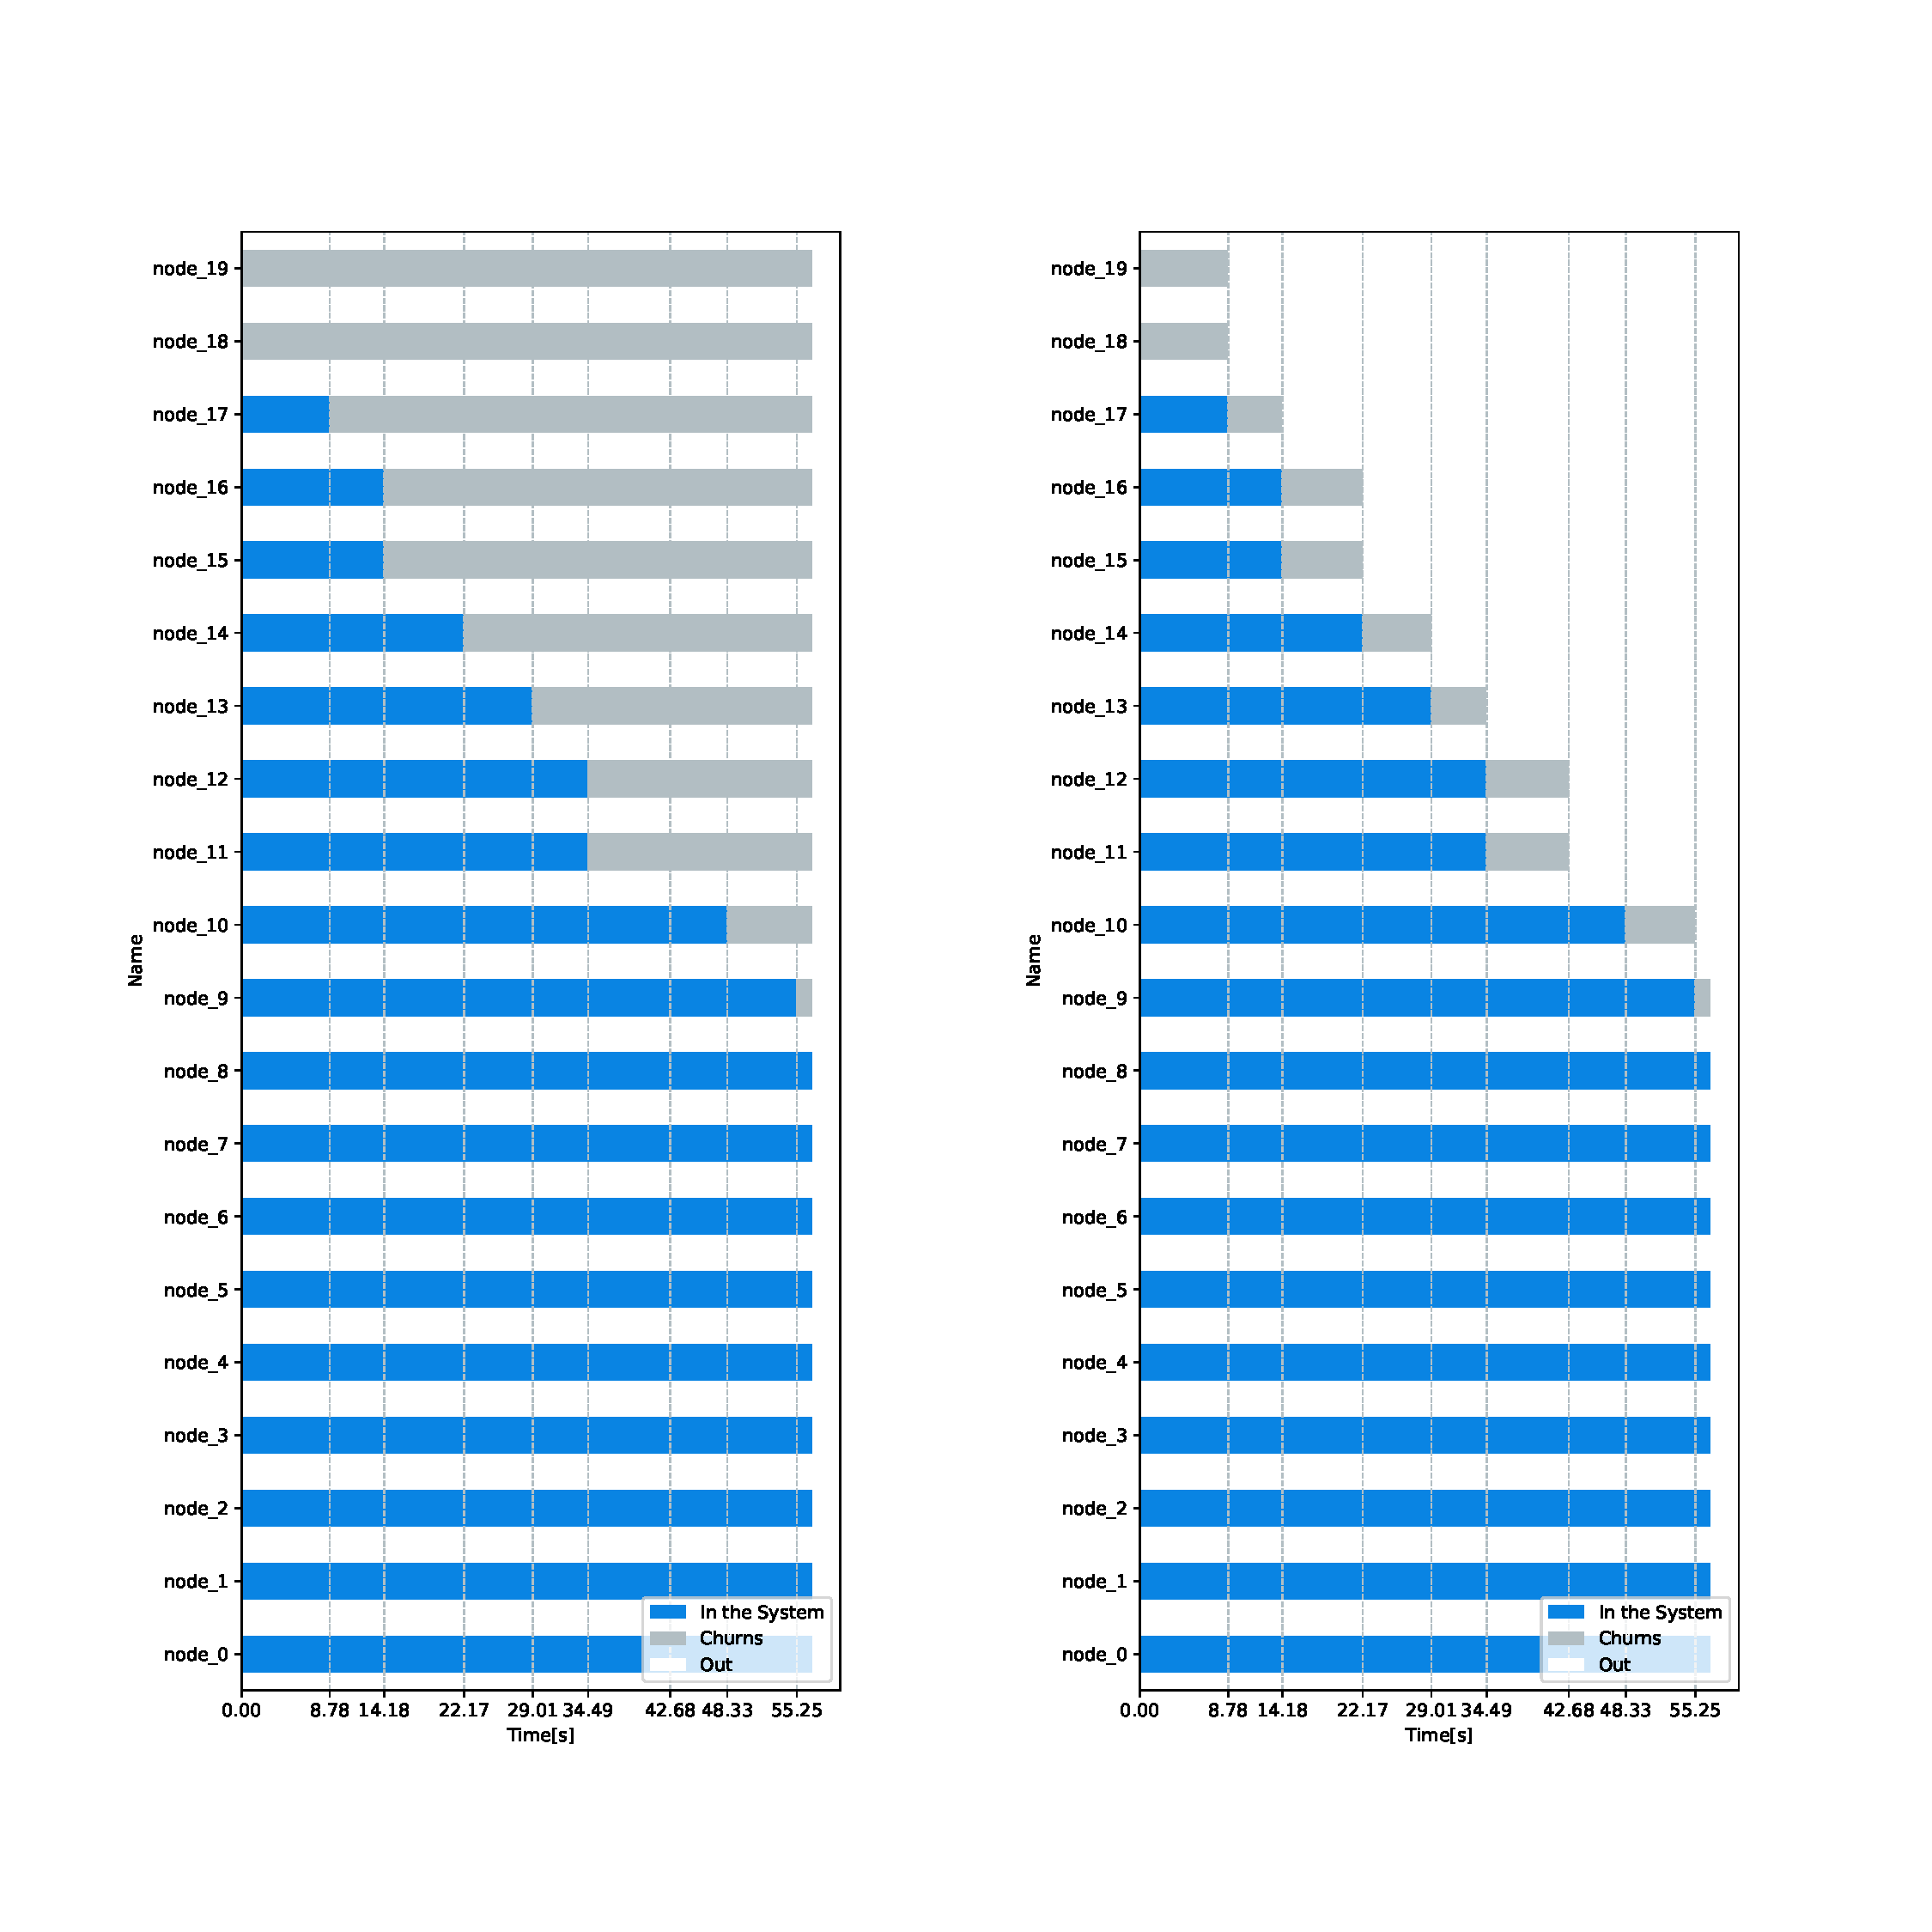
\includegraphics[width=450pt]{figures/ChurnSubplots}
\caption{The simple control plane remove nodes that have left the system. The
    left plot represents the case with a fixed control plane. In this case, the
    nodes that are still alive considers that nodes that have churned are still
    part of the system. On the contrary, with the control plane, nodes that
    churn will leave the system leading to the redrawing of the regions. The
    ticks are placed at the start of epochs.} \label{fig:churn-comparision}
\end{figure}

\subsubsection{Adaptation to Node Movements}
Nodes can move as well, and the latencies between different nodes can change.
If the regions are only drawn at the beginning of the system, then it's
possible that after a while, many nodes have migrated from where they were when
the regions were drawn. This might be a problem. Indeed, the purpose of the
replication was to ensure that in case of a partition, nodes participating in
the same side of the partition should still be able to work. If most of the
nodes have moved, but are still participating in the region of their first
assignment, a partition could happen somewhere in the system leading to failing
regions that should be on the same side of the partition. The control plane
solves this problem as the regions are recreated at each epoch, taking into
account the movement of the nodes, and increasing the partition resistance,
with the movement of nodes.

\subsection{Drawbacks}
This control plane is simple and reaches its objective, but it requires many
resources. Some of the drawbacks of this approach are listed below. 
Some answers to these drawbacks are discussed in \Cref{chap:Improvements}.  

\subsubsection{Control Plane is global}
If the system is replicated in all the regions, the control plane itself is
global. Meaning it could be subject to a partition. In this case, the replicated
system would continue to work, but the control plane could only continue to
work on the side of the Byzantine majority.  On the side of the minority, no
consensus could be reached anymore. Therefore the system will stay stuck at the
same epoch. This is not a major drawback as the main purpose, which is the
liveness of regions that are not split by a partition is guaranteed. However,
the evolution of the system on the side of the minority is not treated by the
control plane.

\subsubsection{Epoch Transition Requires Resources}
Epoch transition requires many resources. Indeed, it needs much
communication for the registration as every node that was
previously on the system should be contacted by every new node. If $\bar{N}$ is
the average number of participants in epochs, then registration requires
$O(\bar{N}^2)$ messages, as every new node has to send a message to every
member of the previous committee. This can be inefficient. 

Then when the registration is done, the protocol as it is redrawn most of
the regions as the algorithm for region creation is reused. This can be
inefficient as well because some transfer of information between old regions
and the new one might be expected.

\begin{figure}[!h] 
\centering
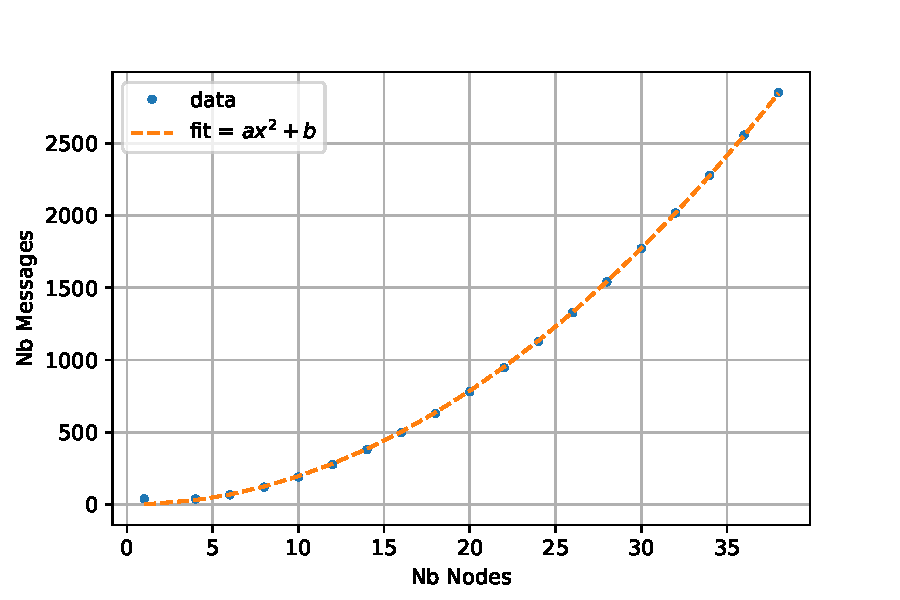
\includegraphics[width=350pt]{figures/messages-plot}
\caption{Growth of the number of messages for one epoch with the number of nodes.}
\label{fig:messages-plot}
\end{figure}

This could be solved by using a random subset of the participants as the
\textit{admission committee}. If $x$ nodes join and a subset of $y$ nodes out
of $N$ are in the  \textit{admission committee}, this could be reduced to
$O(xy)$ messages. This was not implemented due to time reasons, but it is a
simple and straightforward amelioration of the system. 
 
\subsubsection{Omniscience of the Nodes}
Nodes are aware of a lot of information. By design, they are aware of
the list of every other node in the system, their levels, the pings between
each pair of nodes in the system, all the region created and all the region
assignment. The nodes need to be aware of this information so that
every node runs the algorithm for region creation and lands in the same
regions. However, this can be much information to store. Of course, after the
region computation, the nodes could free this memory, but it gives an idea of
how much resource is needed.

\begin{figure}[!h] 
\centering
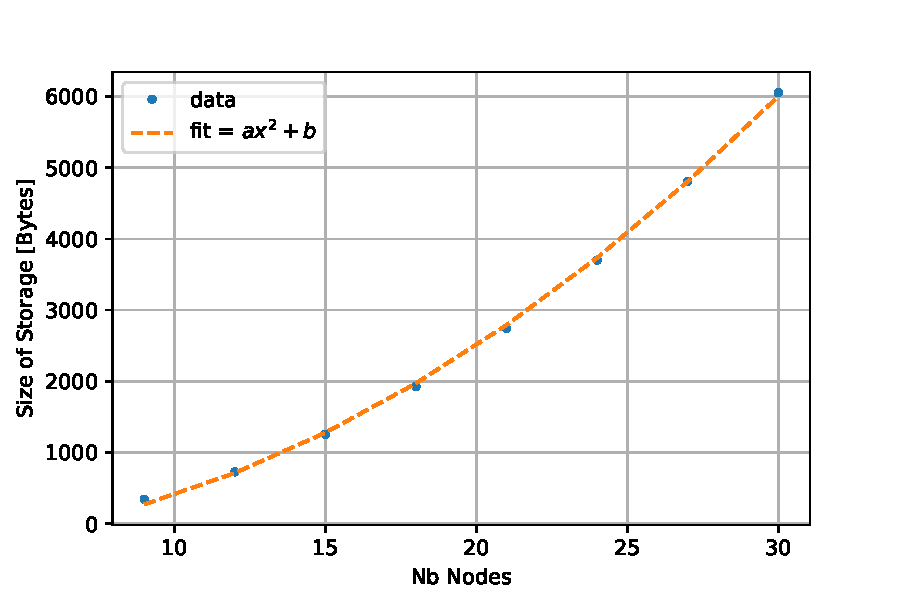
\includegraphics[width=350pt]{figures/storage-plot}
\caption{Growth of the amount of storage required for ping distances for one
    epoch with respect to the number of nodes. } \label{fig:storage-plot}
\end{figure}

\section{Security Analysis}
\subsection{Network Attacks} 
\subsubsection{Man-in-the-middle attacks} \label{MitM}
The messages exchanged during the protocol are listed in the following table
[\autoref{tab:messages-table}].

\begin{table}[]
\centering
\begin{tabular}{m{0.05\textwidth}m{0.25\textwidth}*{2}{>{\arraybackslash}m{0.3\textwidth}}}
\toprule
&\textbf{Message}                       & \textbf{Signature}           & \textbf{Effects of a Sufficient Delay} \\ \midrule
$1.$ & Join request                        & Requesting node           & Request refused    \\ \hdashline
$2.$ &Threshold signature of the request                & Threshold number of the current committee & Request refused    \\ \hdashline
$3.$ &Broadcasting of the Threshold signature             & Threshold number of the current committee & Request refused    \\ \hdashline
$4.$ &Messages for the consensus on the participants,
list of the participants                      & Leader of the current committee     & View Change     \\ \hdashline
$5.$ &List of pings and levels                    & Leader of the current committee     & View Change \\
\midrule
\bottomrule
\end{tabular}
\caption{List of the messages exchanged during the protocol. The signature of
    the message and the effects of a delay are given. }
    \label{tab:messages-table}
\end{table}

As all the messages are signed, if a message is changed, it is noticed by
the receiver, which discards the altered message and asks again to the
sender. Therefore the only effect of a Man-in-the-middle attack is to
delete some of the messages, which can be seen as a type of delay attacks. 

\subsubsection{Delay Attacks}
This protocol is not resistant to delay attacks. It assumes wall-clock
synchronicity between the nodes, which can cause some problems. The effects of
delaying messages are listed in [\autoref{tab:messages-table}]. During the
registration, if the messages are delayed until the start of the next epoch,
then it leads to the refusal of the request, and the node has to create a new
request for the next epoch. If the messages of the leader of the consensus for
the participants of the pings and levels are deleted or delayed, the other
nodes ask for a view change: requesting the next node in the list to start the
consensus again. If attackers manage always to delay the messages of the
successive leaders, it can block the protocol forever.

\subsection{Malicious Nodes}
\subsubsection{Attack on Consensus} If a malicious node is already in the
committee, the only misbehaviour that it can have is to refuse to sign some
messages. Sending forged messages are already treated in \autoref{MitM} as they
are not possible to forge because of the signature. Refusing to sign joining
requests can lead to a failing protocol if the number of malicious nodes is
more significant than the threshold required to get the signature. As the
signature procedure is done using BlsCoSi \cite{Boneh2018}, the registration
process is subject to the same threat. BlsCoSi \cite{Boneh2018} is an efficient
way to implement the \textit{Practical Byzantine Fault Tolerance} (PBFT)
\cite{Castro1999} algorithm which guarantees \textit{safety} and
\textit{liveness} if the system as no more than $f$ faults among $N = 3f+1$
nodes. Therefore it is required to have no more than $f$ malicious nodes. As
the number of nodes in the system evolves with time, it required not to have
more than this fraction of malicious nodes in the system at any epoch. If for
one epoch, the number of malicious nodes is bigger, then they can block all the
consensus, leading to a failing system.  If a malicious node is elected as a
leader of the consensus on the list of participants or the pings, it can decide
not to start the consensus. After a while, another node is elected to run the
consensus (view change), which eventually succeeds if the number of malicious
nodes is low enough.

\subsubsection{Attack on Levels} \label{sec:ControlePlane-Threat-Model}
At the beginning of one epoch, nodes compute their bunch and cluster based on
the pings and the levels that are drawn from a shared public source of
randomness, which is renewed at each epoch. Each node participates in regions
along its bunch. It is important to realize that this procedure is not based on
the action of a node, but just on the fact that they exist at a given place and
a given level, which means that every node has the same view of the system. If
node $A$ has node $B$ in its bunch, then node $A$ is supposed to participate in
a region which is based on the position of $B$ and spans the cluster of $B$,
but $A$ already has all the information to know about this region using only
the pings and levels. Therefore node $B$ cannot use a high level to perform an
action that blocks the system. 

However, if a malicious attacker could take over the lottery process, it could
manage to group the high level in a side of the system, leaving only the
level-zero on the other side. This could lead to an overhead problem which is
described in the next paragraph.  Taking over the lottery process should not be
possible by design. Indeed, the lottery is based on a public source of
randomness which is renewed at each epoch and revealed after the registration
of the levels. Nodes can know the level of other nodes because they base the
computation of their levels on the threshold-signed list they received from the
previous committee. The source must be revealed after registration of the
levels. Otherwise, malicious nodes could try to influence the order of the list
on which the lottery process is based. 

\paragraph{Problem with unbalanced levels.} \label{app:unbalanced-levels}
The problem with unbalanced levels is mainly that a property stated in CRUX
\cite{Basescu2014} is not necessary respected anymore. The property is the
following : Let's call $ARAs_{max}$ the maximum number of regions in which a
node participates. This number is given by : 

\begin{equation} \label{eq:ARAmax}
ARAs_{max} = \log_2(R_{max}/R_{min}) (B \log_B(N)+1)
\end{equation}

Where $B$ is a constant, $N$ is the number of nodes in the system, $R_{min}$ is
the diameter of the smallest region and $R_{max}$ is a diameter that is large
enough to cover the entire network. This ensures that the overhead that is
created by the replication stays reasonable: by design, it is growing
logarithmically with the number of nodes $N$ and with $R_{max}$. We describe
two situations where this property is not maintained, as an argument for
keeping the distribution of levels balanced.

\paragraph{Problem With level-0 Nodes.} \label{app:levels-zero}
Assume that there is a system of $N$ nodes that are all at level 0. If all the
nodes stay at level 0, by construction, they have every other node in their
bunch [\autoref{fig:ClusterBunch-Bunch}]. (Because it’s adding every other node
if their level is not smaller.) After adding $N$ nodes with this process, the
$N$th node participates in $N-1$ region, which grows a lot faster than
\autoref{eq:ARAmax}. This could create an unmanageable overhead.  Therefore one
needs to have higher-level nodes in the middle of levels 0 nodes.  This
justifies the attack on levels that could be done by malicious nodes as
described in \autoref{sec:ControlePlane-Threat-Model}, and the solution
proposed in \Cref{chap:Possible Improvements}.

\subsection{Problem With Too Many Different Levels} Similarly, consider the
case where we have $N$ nodes, and each is at a different level from $0$ to
$N-1$. By design, the node at level $0$ has every other node in its bunch. So
it participates in $N$ regions, which grows a lot faster with $N$ than
\autoref{eq:ARAmax}. This could lead to an unmanageable overhead as well. Of
course, this example is a bit extreme, but it gives guidelines on what could
happen if the distribution of levels is not controlled.

%%%%%%%%%%%%%%%%%%%%%%%%%%%%%%%%%%%%%%%%%%%%%%
\chapter{Improvements} \label{chap:Improvements} %%%%%%%%%%%%%%%%%%%%
%%%%%%%%%%%%%%%%%%%%%%%%%%%%%%%%%%%%%%%%%%%%%%

This section proposes some improvements to the simple control plane protocol.
They are supposed to address the drawbacks of the simple protocol, and each
improvement is illustrated in a Strawman model. Finally, an advanced version of
the control plane that uses a region creation algorithm based on time/space
graphs is proposed. 

\section{Strawman 1 : Locarno Treaties} \label{Locarno}

\begin{figure}[!h] 
\centering
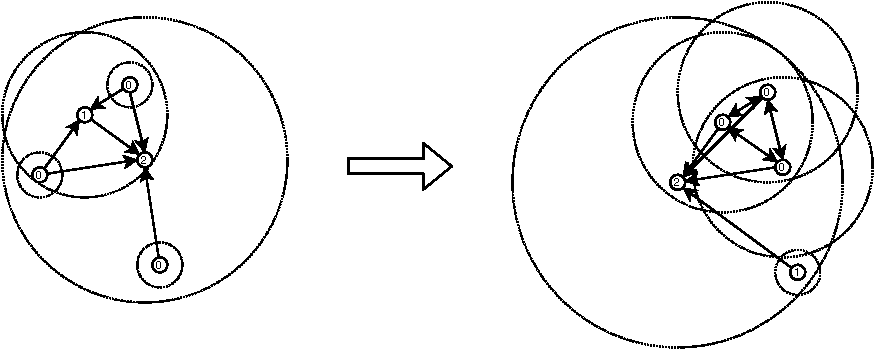
\includegraphics[width=300pt]{figures/LocarnoTreaties-Redrawing}
\caption{Redrawing the levels at each epoch can lead to very different version
    of the system. This is what is improved by the Locarno Treaties.}
    \label{fig:LocarnoTreaties-Redrawing}
\end{figure}

Following the First World War, it was decided that the borders of Germany
should remain fixed. The Locarno Treaties defined some of these borders. The
idea of this Strawman model is to do the same by limiting modifications of
regions from one epoch to the next. The idea is to use a deterministic set of
rules, based on the ping, the registrations and the map of the previous epoch
to create the map of the current epoch using the fewest modifications possible.
Registration is still global, and each node has all the information about the
memberships of every node. Then from one epoch to another, the purpose is to
keep as many unchanged regions as possible. The obvious idea to reach this goal
is to let the nodes keep their levels from one epoch to the next. However, this
introduces some overhead problems.  These are described in the next section.

\subsection{Rebalancing the Levels} \label{rebalancing} Conserving the levels
is the way to go, but maintaining levels can lead to unbalanced systems.
Consider a system with 200 Nodes at epoch 1, with the repartition given in
\autoref{example-lottery}. If from epoch 1 to epoch 2, 100 level-0 nodes leave
the system. The remaining system would contain 80 level-0 nodes instead of 90. 

Unbalanced systems can lead to various problems. Some examples are given in
\autoref{app:unbalanced-levels}. The lottery process presented in
\autoref{sec:common-tools} is slightly modified in this section to allow the
adaptation of the levels. The total number of participants $N$ in the system is
known after the registration, and as the probability $P$ is given, it is
straightforward to compute the expected number of nodes that one should have at
every level as it is mentioned in \autoref{example-lottery}. 

Instead of drawing the levels directly from a randomness source, nodes 
draw a random number from this source between 0 and 1
[\autoref{fig:sketch-new-levels}]. All nodes can deduce what number the others
draw deterministically from the registration list and the public source of
randomness. The highest level goes to the node, which has drawn the highest
random number. Levels are given according to the drawing in descending
order. Each node that stays in the system keeps its random number from when
it joined the system, and new nodes get fresh random numbers. This does not
guarantee that nodes keep exactly the same levels, but, most of the time, it
will be the case.

\begin{figure}[!h] 
\centering
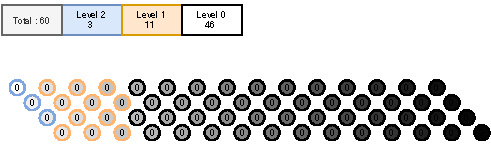
\includegraphics[width=400pt]{figures/Lottery-Locarno}
\caption{Sketch of the new method for drawing the levels. The fill property of
    each node represents the number that was drawn from 0 (black) to 1
    (white).}
 \label{fig:sketch-new-levels}
\end{figure}

\subsection{Motivation for Keeping the Levels} This section describes the
reasons for keeping the levels. It is useful to look in detail at what are the
consequences of the movement of a given node on a given fixed node, to
understand what are the effects on the global system. Then some precise
examples of the evolution of the system are treated as well. The hypothesis in
this analysis is that the nodes keep the same levels using the new lottery;
this is assumed to make things simple. But we have to keep in mind that the
lottery process might allow nodes to change levels for keeping the system
balanced.

\subsubsection{Effects for a Fixed Node} The point of view of one node that
stays fixed in the system is considered, the goal is that the node can keep
most of its region assignments. Other nodes might join, leave or move, and this
can result in changes either in its cluster or in its bunch. 
[\autoref{fig:LocarnoTreaties-Leaving-cluster}]. 

\paragraph{Nodes Leaving the Cluster} This can shrink the cluster of the fixed
node. As the regions created by a given node stops when the radius covers the
whole cluster, this might lead to the deletion of some regions. This does not
change the region assignment, and the nodes can still keep the replicated system
of the previous epoch running. 

\paragraph{Nodes Joining the Cluster} On the contrary, if nodes join the
cluster of the fixed node, this might lead to the creation of an additional
region to cover these extra nodes. The node then replicates its system to
the newly created regions. So the fixed node keeps the regions it created,
which was the goal, and eventually add some to cover its cluster.  By design,
these joining nodes could be part of the bunch of the fixed node as well, but
this case is treated in another paragraph.

\paragraph{Nodes Leaving the Bunch} Nodes participate in all the regions in
their bunch. Eventually, they participate in a region that covers the
whole system. If a node left the system in the bunch, this leads to a region
centered around a point that is not in the system anymore, and this assignment
might be forgotten. 

From a fixed node, if another node leaves its bunch, it can have an effect to
add other nodes in its bunch, leading to more region assignment. And in some
cases, to more nodes in its cluster, leading to region growth. 

\begin{figure}[!h] \centering
  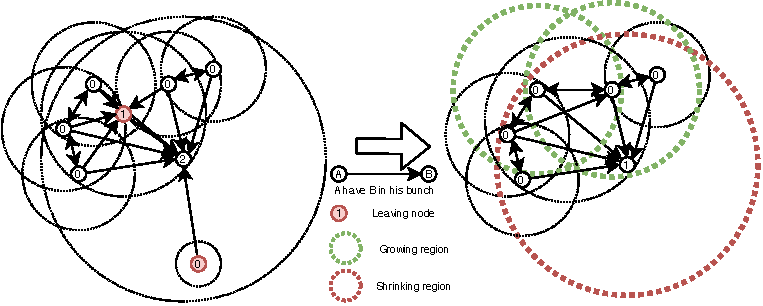
\includegraphics[width=300pt]{figures/LocarnoTreaties-Leaving-cluster}
  \caption{A leaving node changes assignments of other nodes but keeps the
  same regions. }
\label{fig:LocarnoTreaties-Leaving-cluster} \end{figure}

\paragraph{Nodes joining the Bunch} If nodes are joining in a bunch, this leads
to additional region assignment. 

\subsubsection{Rules for other nodes} The point of view of a fixed node in the
system was treated. The other nodes have yet to be reviewed. The
question is how to integrate moving or joining in the system while keeping the
system balanced. 

\paragraph{High-Level Moving Node} Assume that going from epoch $i$ to $i+1$,
one of a relatively high-level node has gone from one place to the other end of
the system. As nodes can keep their level, it changes some of the assignments,
but most of the regions are maintained. 

\begin{figure}[!h] 
\centering
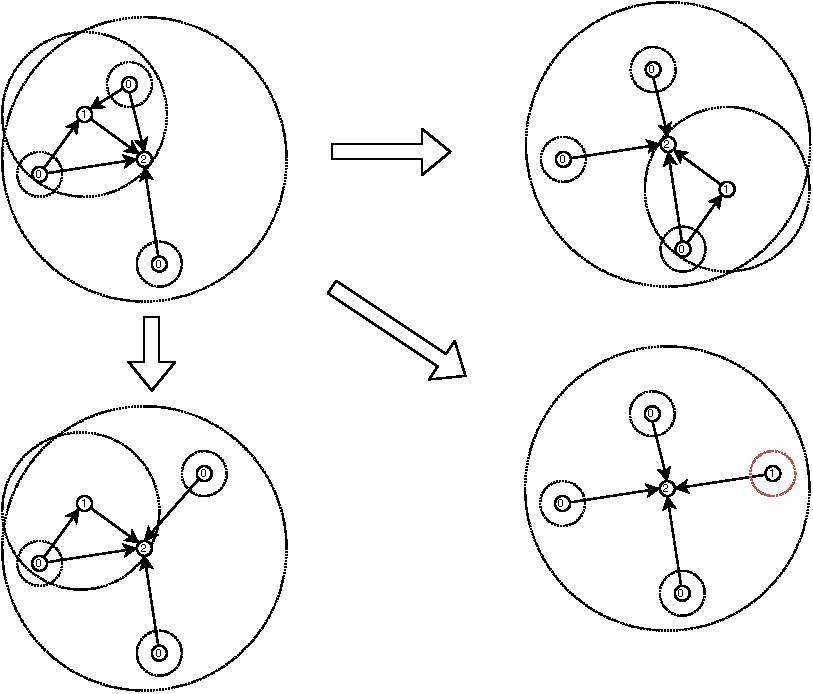
\includegraphics[width=300pt]{figures/LocarnoTreaties-Moving}
\caption{A moving high-level node keeping its levels is changing assignments of
    other nodes but keep the same regions. }
\label{fig:LocarnoTreaties-Moving}
\end{figure}

This seems to indicate that movement should not be a problem. There is a
slight difference between that situation and changing the levels at each
epoch. As each node can keep its copy of the underlying system working in its
region. If the levels are changed, communication might be needed to transfer
data from one region to another. This communication overhead is reduced in
that situation. 

\paragraph{Low-Level Moving Node}
The consequences of a low-level moving node are less important than a
high-level moving node as most of the other nodes won't have it in their bunch.

\paragraph{Levels of Joining Nodes}
One can think that the levels of joining nodes might have a big influence on the
system; this part tries to illustrate what might happen. The joining nodes can
lead to the growth of one region or the creation
of regions. The effects of the level of joining nodes are illustrated in
[\autoref{fig:LocarnoTreaties-Insertion-close}][\autoref{fig:LocarnoTreaties-Insertion-far}].

\begin{figure}[!h] 
\centering
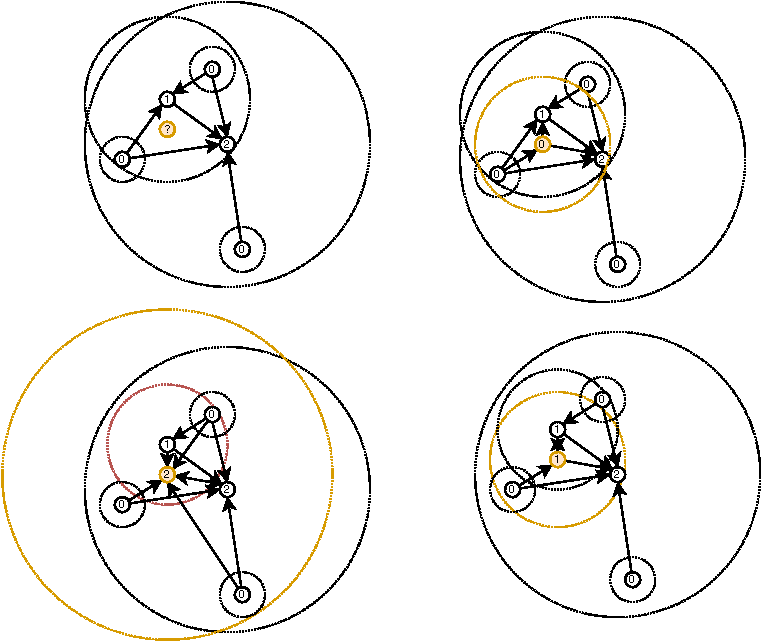
\includegraphics[width=300pt]{figures/LocarnoTreaties-Insertion-close}
\caption{Keeping the same level leads to smaller changes when a node enter the
 system close to other nodes. } \label{fig:LocarnoTreaties-Insertion-close}
\end{figure}

\begin{figure}[!h] 
\centering
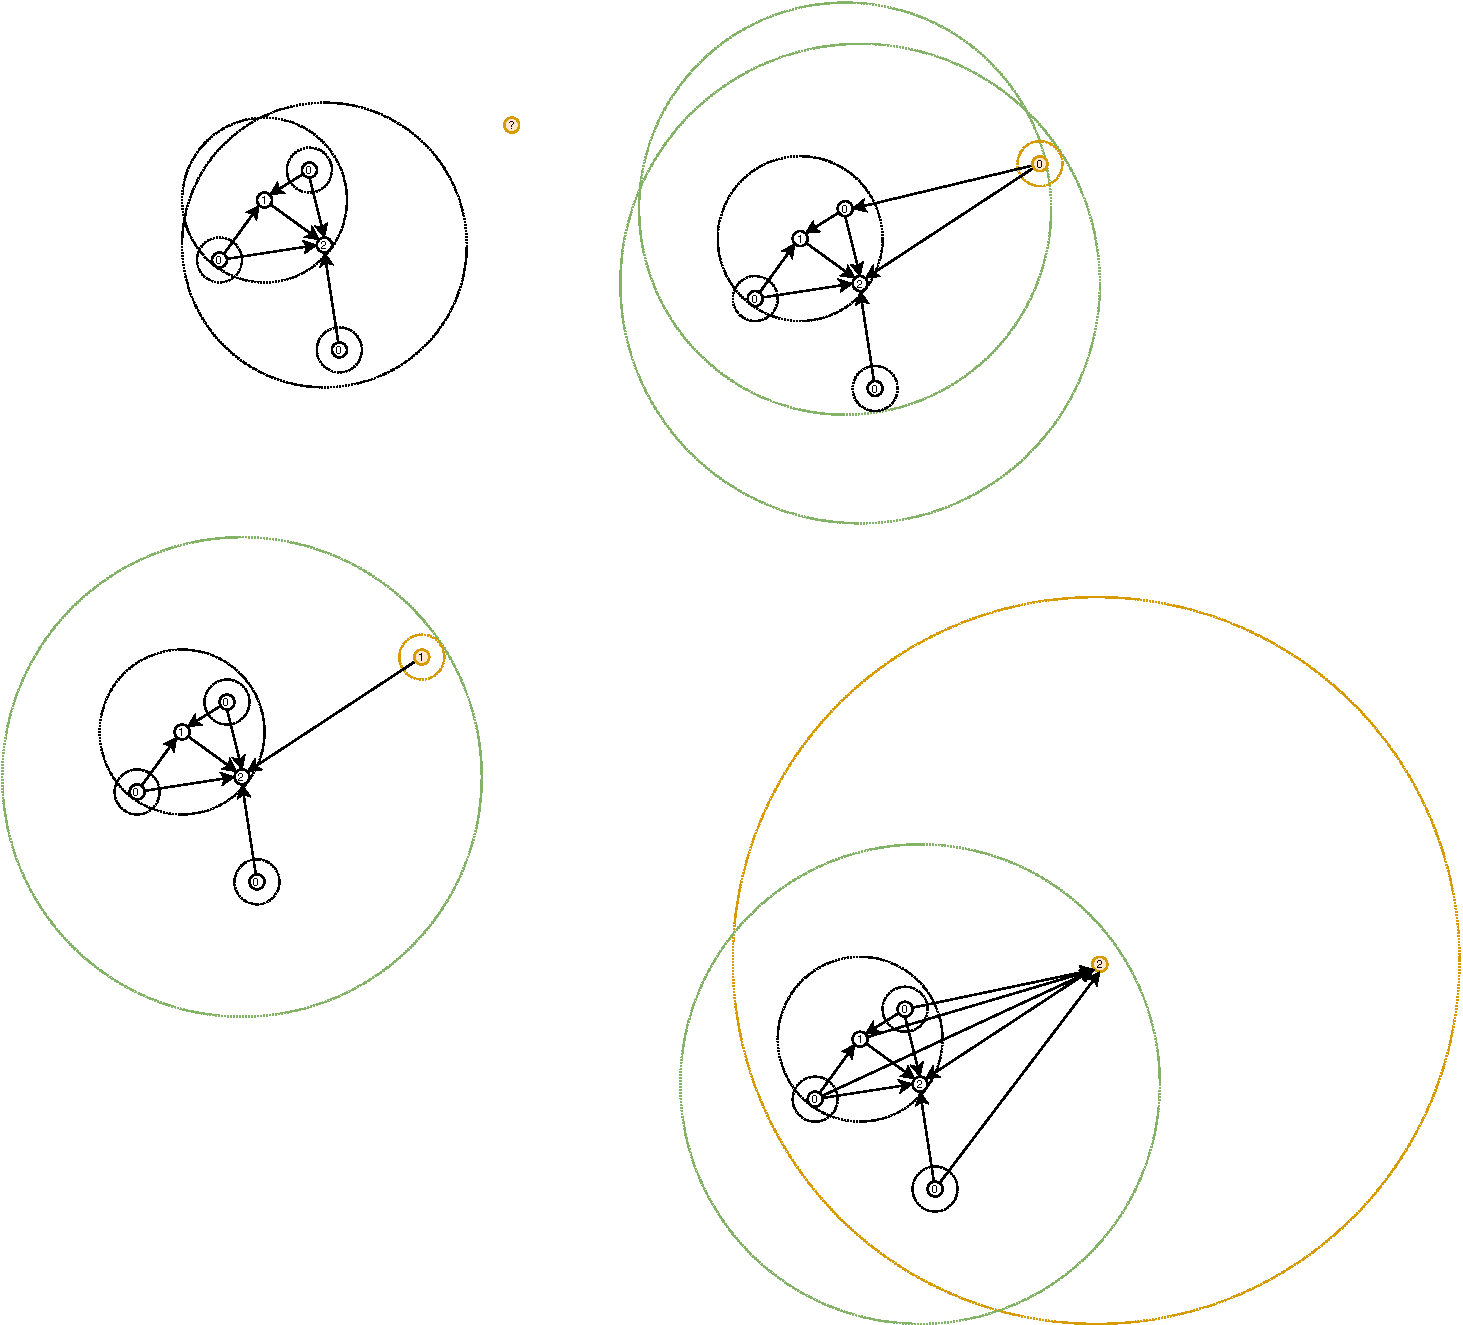
\includegraphics[width=300pt]{figures/LocarnoTreaties-Insertion-far}
\caption{Keeping the same level leads to smaller changes when a node enter the
 system from far away. } \label{fig:LocarnoTreaties-Insertion-far}
\end{figure}

\subsection{Protocol}
The protocol is mostly the same as the simple control plane protocol
[\autoref{fig:registrationprotocol}]. The main difference is the level
assignment which follows the new algorithm described in \autoref{rebalancing}. 

\subsection{Threat Model}

Attackers can target the new lottery process. If one malicious node decides to
attack the system alone, it does not create too disastrous consequences, as it
is presented in \autoref{sec:ControlePlane-Threat-Model}. Another attack could
be that malicious nodes exit and reenter the system at each epoch until they
manage to get a good number from the lottery. Then when it achieves to get a
right level, they collectively move to one side of the system leaving good
nodes all at level-0 in the middle of the system. This creates a slight
overhead for the good nodes as the region’s assignment increase for the level-0
nodes.  But this attack seems to cost a lot of resources and coordination for
the attacker to generate a small overhead on the size of the participants. Some
defence mechanisms can be set up to ensure that levels are geographically
distributed over the whole system, they are described in more details in
\Cref{chap:Possible Improvements}.

\subsubsection{Quantifying the Effect of Locarno Treaties}
The goal of the new protocol is to keep most regions and region assignments
following the evolution of the system. A detailed comparison is made. The
system starts with a fixed number of nodes and evolves with nodes moving,
leaving and entering the system. A quantity is chosen to evaluate the
difference between the system from one epoch to the next. The quantity is
defined as follows: the list of participants in the system is taken sorted by
name. The bunch and cluster are seen as a set of nodes. The number of
difference between a set A and a set B is defined as follow :
\begin{equation}
\# \textrm{Diff}(A,B) = \#(A \cup B - A \cap B )
\end{equation}
where $\#$ means the number of elements in the set.

Then for each node, the number of difference between their bunch and cluster at
epoch $i$ and their bunch and cluster at epoch $i+1$ is computed. If a new node
enters the system, the differences between their bunch and cluster and an empty
set are computed. Same if a node leaves the system. The idea is that with this
new protocol, the total number of differences should be reduced.  The results
of the experiment can be seen in [\autoref{fig:LocarnoTreaties-differences}].
They are averaged on 100 different experiments for each lottery. The number of
nodes at a given epoch is kept constant to ensure that the experiments are
comparable. The system starts with 4 nodes and then, 2 additional nodes are
joining at each epoch. The following model for the nodes is taken: The size of
the system is $(300, 300)$. Each node starts at a uniformly random position in
the system. Then, at each epoch, every node has a probability of $20\%$ to make
a local movement, and a probability of $10\%$ to be teleported at another place
in the system. A local movement changes the current position $(X ,Y)$ by adding
to X and Y two different uniformly random numbers between $(-10, 10)$.
Teleportation sets the position of a given node to another random position in
the system. The pings between two nodes are defined as a linear function of the
distance. The maps and details of one given experiment are given in
\autoref{app:LocarnoTreaties-data}.

\begin{figure}[!h] \centering
  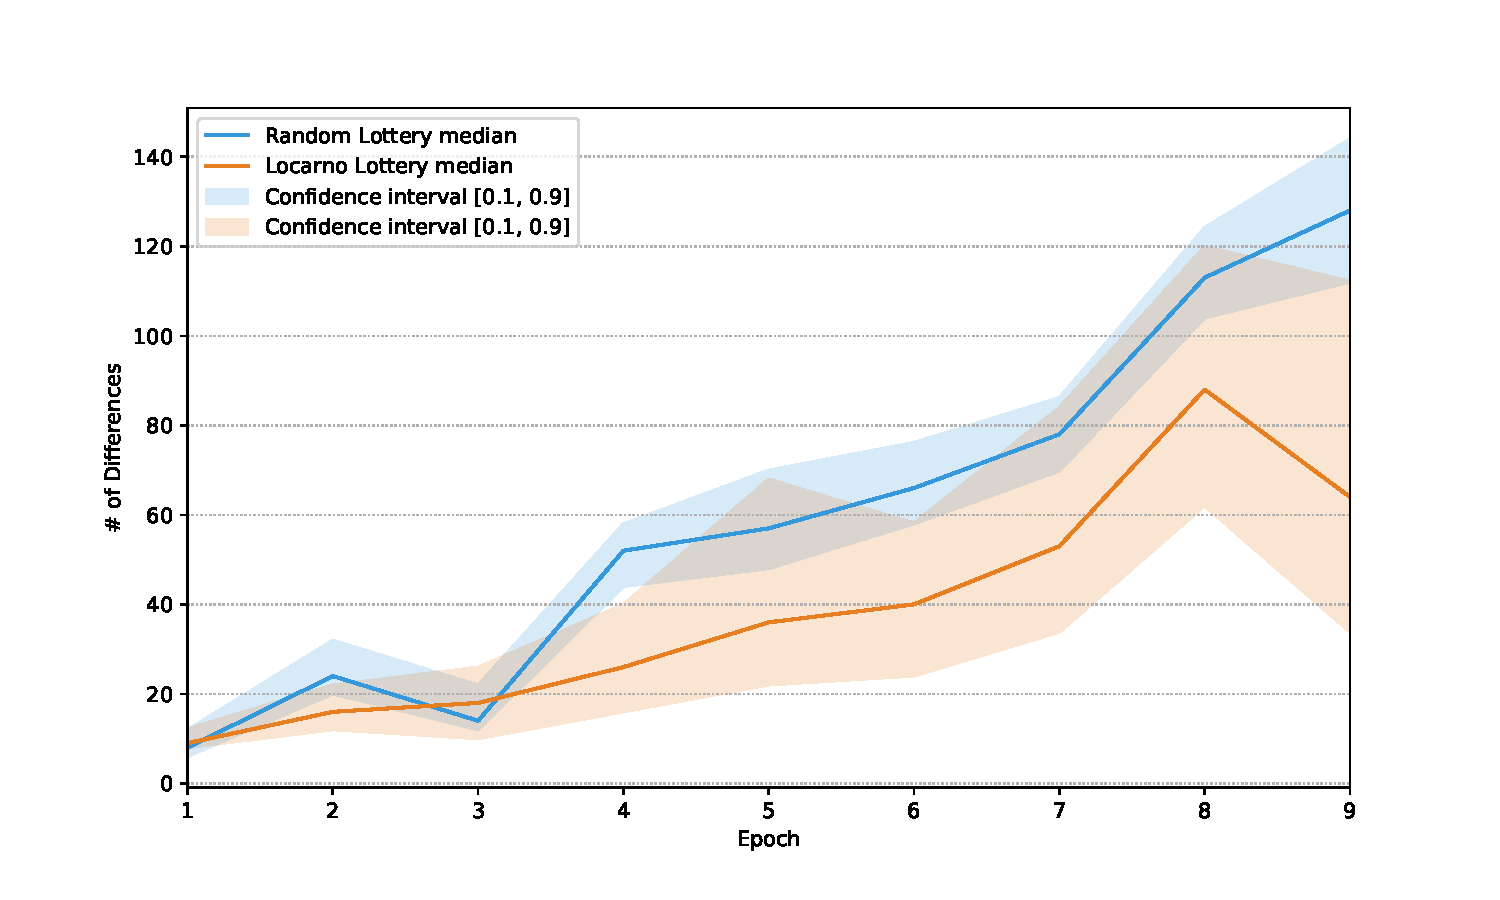
\includegraphics[width=400pt]{figures/LocarnoTreaties-differences}
  \caption{Graph of the number of differences between maps from one epoch to
  the next using the random level assignments or the one defined in Locarno
  Treaties. Maps and details of the system are given in
\autoref{app:LocarnoTreaties-data}. } \label{fig:LocarnoTreaties-differences}
\end{figure}

The figure shows that globally the Locarno Lottery leads to less difference
from one epoch to the next. However, the results of the random lottery seem to
have less variance. This might be due to the teleportation factor as if nodes
move too much, the system becomes equivalent to the random lottery. But
overall, this small amelioration led to the reduction of the differences from
one epoch to the next.

\section{Strawman 2 : Fog of the War} \label{sec:Fog-of-the-war}

Each node of the system has a different view of the world at a given time,
depending on its place in the system and its interactions. Again the idea is
that one node should only be aware of the information it needs to perform its
actions. Correspondence can be made with the fog of war of some traditional
real-time strategy video game, where each player have its view of the system,
based on where he is now (light), where he was in the past but cannot see now
(fog) and what he has not already seen (dark) [\autoref{fig:fog-of-the-war}].
Each player view evolves through space and time accordingly.

In the context of the game, the advantage of this view is that it hides the
adversarial strategy. Indeed each player can move his troops, and the only
information about that that another player can have is if he has himself a unit
in the same region. In the context of our system, this view
hides most of the information that is not relevant to one node but allows it
to perform its operation without the storage and communication overhead. 

The design of this Strawman is the following. Each node declares a position
during the registration, and other nodes compute their bunch and cluster
according to this declared position. This is different from the two first
protocols were each node announced his pings to every other node in the system.
Each node will, therefore, be able to compute their bunch and cluster based on
these declared positions. A random committee of checkers is elected after the
registration process to ensure the correctness of the system. These checkers
perform some tests (pinging other nodes of one region) and publish the results. 

\begin{figure}[!h] 
\centering
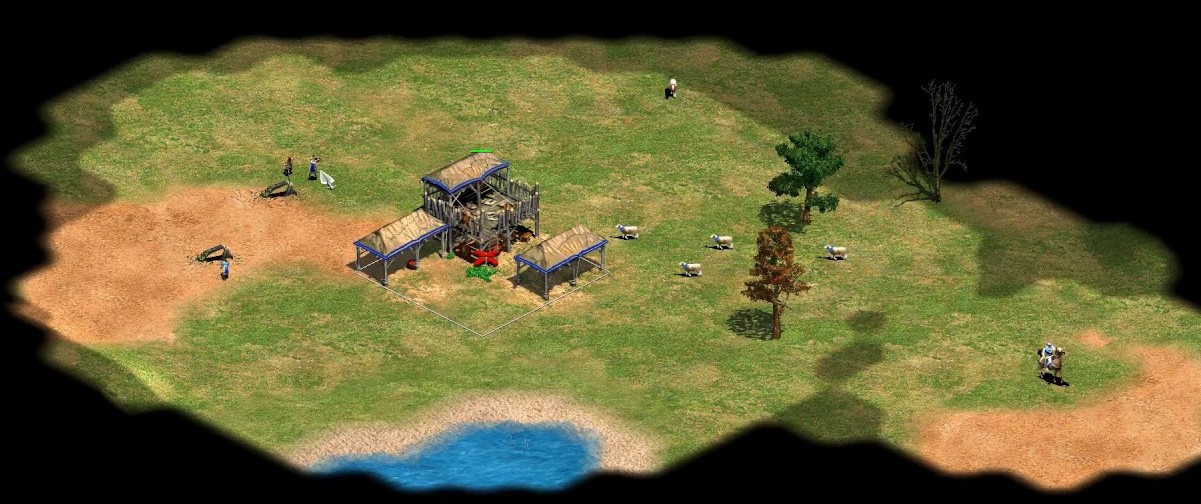
\includegraphics[width=400pt]{figures/fog_of_war}
\caption{Fog of war representation in a classic real-time strategy video game \cite{ageofempire1999}. }
\label{fig:fog-of-the-war}
\end{figure}

\subsection{Purpose : Reducing the Need of the Consensus on Distances}
The protocols presented in the Simple Control Plane protocol and the Locarno
Treaties still need consensus on the distances between all nodes in the system.
This can be cumbersome as the number of nodes increases in the system in
$O(N^2)$, where $N$ is the number of nodes. Consensus might become too costly
for that reason.

The idea is to change that consensus with a declared position and a random
committee of checkers. The question is still: how to choose the committee? If
sampled randomly, the chances are big that the selected nodes are far away
from the node that they are supposed to check, and above a certain threshold,
the correlation between pings and distances are not satisfactory
\cite{Katz-bassett2006}. Therefore the committee of checkers can be selected to
be the $n$ closest nodes based on the declared distances. And $n$ can be
adapted to increase if one node does not pass the checks. 

If a node does not pass the checks, it either means that this node is faulty or
that the number of checkers is constituted of a majority of malicious nodes.
One can solve the second problem by increasing the number of checkers $n$, and
progressively a majority of honest nodes should have checked the node. It the
pings still does not match what the node declared, then that means the node
itself is faulty. 

\subsection{Protocol}
The protocol is mostly the same as the simple control plane protocol
[\autoref{fig:registrationprotocol}]. The only difference is the consensus on
the pings which are now replaced by a declared distance, which is announced
before the level assignments,  and a round of checks and announce of the checks. 

\subsection{Attack on Protocol}
Another question can be, what are we supposed to do with a node that is not
passing the tests? First, it is important to notice that it won't change the
view that all nodes have of the system, as nodes use the declared distance to
compute their bunch and cluster. If used with the Locarno Lottery, a malicious
node could use that system to declare a fake position and virtually go to a
strategic place where it can unbalance the system. This is what one may want to
avoid. 

Two different approaches are considered to solve this problem, the first is to
exclude the malicious node from the system, but it might lead to the redrawing
of a certain number of regions. Another strategy could be to define the
position of the faulty node with an approximation based on the ping. If we have
the position of the other nodes and we fix the location of the unknown faulty
node, one might do that by computing the intersection between the circles based
on the pings. This triangulation strategy
[\autoref{fig:triangulation_strategy}] can block one faulty node to reach the
desired position. This strategy is imperfect for two reasons. First, the
Internet suffers from triangle inequality violations \cite{Lumezanu2009}, and
second, it is possible that the circles based on the pings do not intersect at
the same point. In that case, one has to consider what could be the position
which satisfies most of the constraints that are given. But this was not
designed due to time reason. An analysis of the triangle inequality violations
was made by Pantea Karimi in another project \cite{PanteaKarimi2019}.

\begin{figure}[!h]
\centering
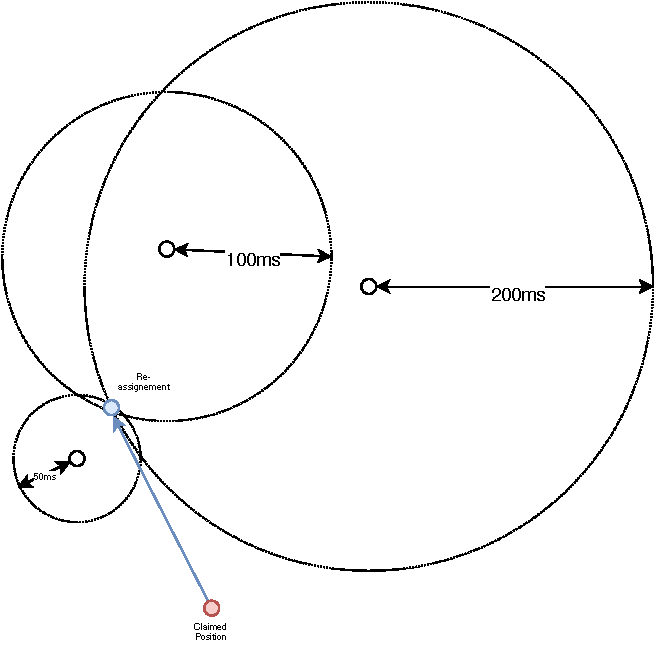
\includegraphics[width=300pt]{figures/triangulation_strategy}
\caption{Triangulation can be used to reassign the position of a malicious
node.}
\label{fig:triangulation_strategy}
\end{figure}

As nodes can announce a position, which is checked in priority by close nodes,
with this protocol, if there is a sufficient number of malicious nodes, they
can declare that they all live in a neighbouring region and validate each
other.  This means that regions with a majority of malicious nodes could be
created. But that was already allowed with the other protocols. This means as
well that these nodes participate in regions, from which they are actually far
away. Thus this will break the latency assumption of one region.  There is no
simple solution to this problem, but that fact has no essential consequences on
the system so it seems to be an acceptable weakness.

\section{Discussion : Space/Time Interaction distance} One of the principal
reasons to split the system based on locality is because of most regular
transactions between people are local. Therefore one wants to ensure that in
case of a global partition, most of the transactions can still be processed
flawlessly. The first idea for the locality was the
following. As there should be more interaction in local regions, they can be
processed locally. This means that by using locality, the real goal is to
maintain the interactions between the nodes. In that case, the space metric is
used to get an insight into the number of interactions between nodes. And this
is a reasonable approximation, but it might be worth it to try to quantify
these interactions directly. 

This goes in an orthogonal direction that the first goal of CRUX and Nyle.
Indeed this part does not try to create regions based on the latency or the
availability, but on the concept of interaction between nodes. This could help
if cross-region interactions are creating some overhead, and this can be the
case depending on the underlying system. With the new proposed distance, nodes
that interact often would be put in small regions.

\subsection{Interactions as a Distance on Space/Time Graphs}

If one wants to leverage the locality of interactions to build regions, it
might be worth it to investigate the following case. Imagine that some nodes
$A$ and $B$ interact often, but they are not part of the same local region. By
design, there is a bigger region in which they interact, and each of these
interactions should pass through this bigger region. One property that might be
useful is that these frequent interactions should have an impact on the system
leading to the creation or update of a region to include the interacting nodes.
If the metric that defines distance is changed from kilometers (or milliseconds
if pings are used to approximate distance) to "interactions". One should be
able to redraw the whole system based on that and to apply Crux to create
regions. Now how to define this metric? Let's try with the following definition
of distance :


$\forall A, B \in S$
\begin{equation} \label{definition-distance}
 d(A,B) = \frac{1}{ \mathrm{\#\ messages\ between\ A\ and\ B\ per\ unit\ of\ time} } 
\end{equation}
Where $S$ is the set of nodes in the system.

It is interesting to note that this quantity has the property of a distance but
not of a metric \cite{Greenhoe2016}. The properties of a metric and distances
are listed below.  Indeed for the first property, if we define that the number
of messages that one node sends to itself is infinite, the distance from one
node to itself would be zero. For the second property, the number of messages
is positive meaning that the distance is always positive. For the third, the
interactions are counted as symmetric (if $A$ is sending a message to $B$, we
count that as an interaction between $A$ and $B$).  But for the fourth, the
triangle inequality is not respected, and that is a problem indeed one should
notice that if $A$ is close to $B$ and $B$ to $C$ but $A$ and $C$ may never
interact therefore are "far from each other".  

\paragraph{Properties} The properties of a metric are $1, 2, 4$ which implies
$3$. The properties of a distance are $1,2,3$ but not necessarily $4$
\cite{Greenhoe2016}. In the case of the interaction distance
\autoref{definition-distance}, $4$ is not respected.

$\forall A,B \in S$
\begin{enumerate}
\item $d(A,B) = 0 \Leftrightarrow A = B$
\item $d(A,B) \geq 0$
\item $d(A,B) = d(B,A)$
 \color{red} \item$d(A, C) \leq d(A,B) + d(B,C)$ \color{black}
\end{enumerate}

\paragraph{Example : Swiss rail network}
A parallel can be made with the Swiss rail network. Indeed in some cases, it is much
faster to take a train from $A$ to $B$ and then to take a train from $B$ to $C$
than taking a bus from $A$ to $C$ [\autoref{fig:CFF-map}][\autoref{fig:CFF-NewDistances}] . 

\begin{figure}[!h] 
\centering
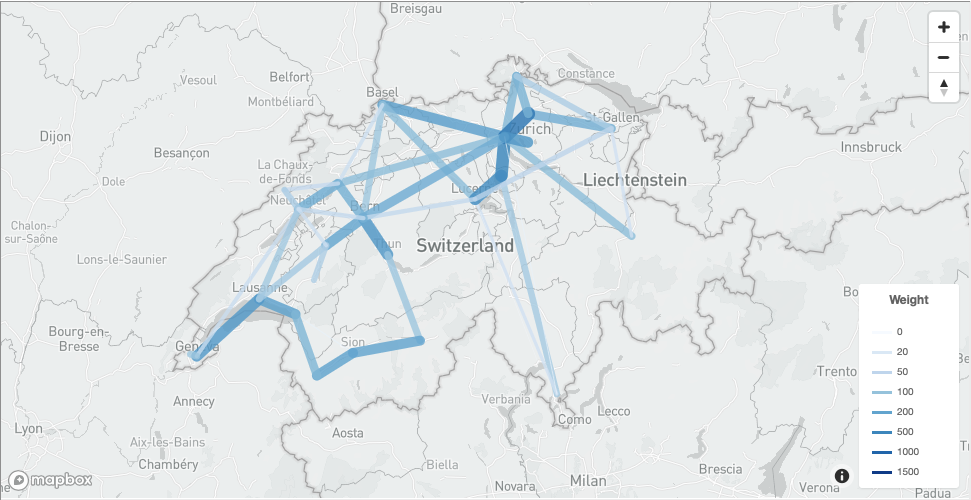
\includegraphics[width=450pt]{figures/mapCFF}
\caption{Map of the train network in Switzerland, line-width is proportional to
    the number of connections per day. Three criteria were held for the
    selection of the cities: size, if they are a capital and my own
    preferences. There is an edge between two cities if there is a direct
    connection in the dataset. This map was done using a Python API
    \cite{MapBox} and is based on public data \cite{OpenData}. }
    \label{fig:CFF-map}
\end{figure}

\begin{figure}[!h] 
\centering
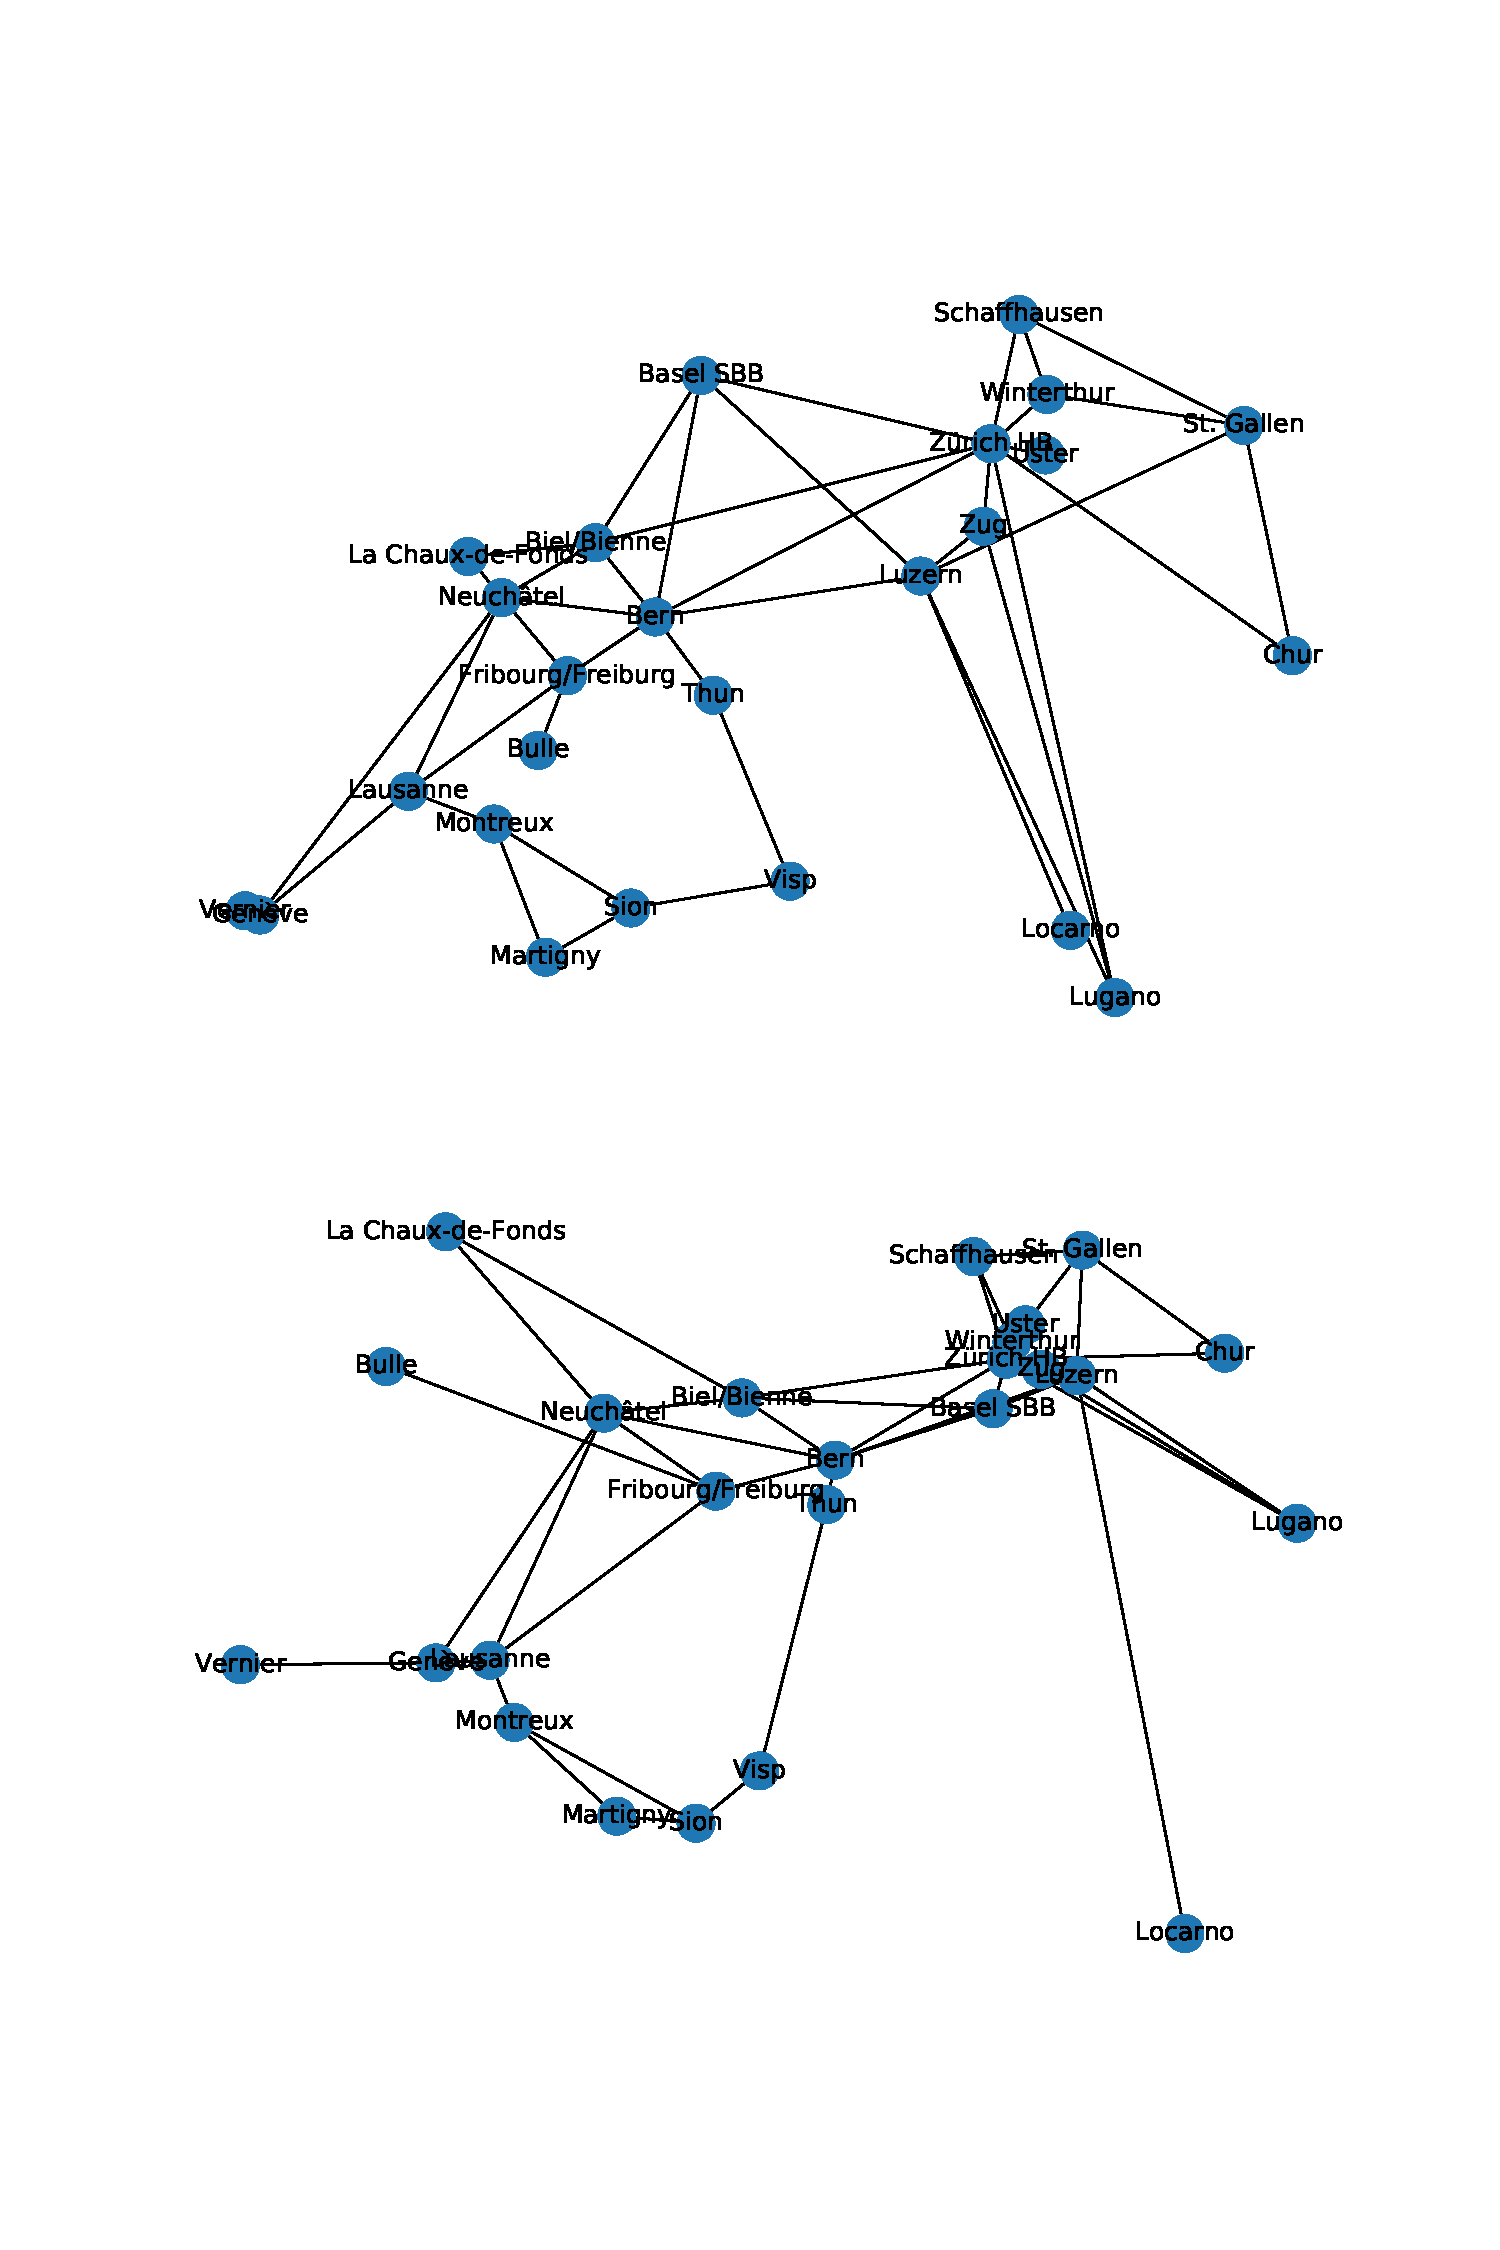
\includegraphics[width=350pt]{figures/CFF-NewDistances}
\caption{The train network is drawn again, using the regular distance first. In
    the second figure, the graph is displayed using the interaction distance as
    force in a force-directed graph. Ensuring that nodes that are close with
    regard to the interaction distance are close on the graph.  Three criteria
    were held for the selection of the cities: size, if they are a capital and
    my own preferences. There is an edge between two cities if there is a
    direct connection in the dataset.} \label{fig:CFF-NewDistances}
\end{figure}

The fact that this new quantity is a distance and not a metric does not create
a problem in our case. Indeed all nodes are considering their distances
directly to all the other nodes in the system. Before, nodes were required to
compute their pings to any other node in the network. Replacing that with the
interaction distance does not change anything. Triangle inequality could be
useful if one was trying to find a path from $A$ to $B$ and was considering
going by different other nodes to arrive at its goal. In our case, this is not
the case, and the hypothesis is that nodes have a one-to-one communication
system.  Therefore it's only required to know the distance between any pair of
points to be able to draw a map of the system. Indeed if nodes are given
levels, and every node knows the pairwise distance to every other node, then it
is possible to compute the bunch and cluster of every node.

\subsection{Finding Meaning}
To understand better what this distance means, some examples are
considered. We want to understand what it means to move with that new distance as
well as joining and leaving the system. 

\paragraph{Movements for Nodes With Interaction Distance}
It is easier to understand what it means to move in that space by looking at
the relative distance between nodes. Imagine that node $A$ gets closer to node
$B$ but away from $C$ in that space. That means that the interactions between
$A$ and $B$ increase and on the contrary that the interactions between $A$ and
$C$ decrease.

\paragraph{Joining nodes with Interaction distance}
If a node joins the system and starts to interact with others, this can be
viewed as a node coming from infinity and getting closer to other
nodes.

\paragraph{Churning nodes with Interaction distance}
If a node churns and stops answering the other, this can be interpreted as a
movement in the interaction space. It is equivalent as if the churning nodes moved
to infinity.  

\paragraph{"Regions" With Interaction Distance} \label{par:section-example}
The concept of the "region" is harder to conceive with that new notion of
distance. It might be useful to use the parallel with the Swiss rail network
\autoref{fig:CFF-NewDistances}, let's imagine a node at EPFL and try to
conceptualize what might correspond to the equivalent of "local", "regional"
and "global regions". The "local" region might be depicted with what places can
be reached within 15 min of public transportation. As the frequency of some
lines, e.g. the metro, are much higher than some bus lines, the places that are
reachable by this means of transportation would be considered as local. At the
regional level, it might be what places are reachable within 1 hour of public
transportation. The global region still covers all the nodes.

\subsection{Justification to Replace the Locality}
Changing the distance from the regular one to interactions might have some
implications on the property that we want to keep in the system. 

\paragraph{Partition Resistance}
Even more than preserving working regions composed of geographically close
nodes, it might be more interesting to preserve the set of nodes that have many
interactions. Since these are perhaps the nodes that are doing the most
operations of the system. This justifies the use of this new distance.

\paragraph{Region Validation for Transaction}
One problem that Nyle wanted to solve was region validation to allow fast
processing of transactions. This is still possible in that case. However, the
region does not correspond to the same anymore. But they would correspond to
the example depicted in \autoref{par:section-example}. This might be acceptable
for a client. 

\subsection{Protocol}
The protocol is the same as the one described in Locarno Treaties in
\autoref{Locarno}. The only difference is that the distance is replaced by the
new distance [\autoref{definition-distance}]. The computation of the number of
messages is done in the following way: each node keeps track of the count
of messages it receives from other nodes between epochs, and post the results
at the beginning of the next epoch instead of the pings. Each node is able then
to compute the new distance, and the algorithm for regions can be used
directly. In the first epoch, as nodes did not have the time to interact a lot
with each other, the map of the system will be very regular with the same
distance between each node. One assumes that because of the underlying system,
nodes will start to interact more with a small subset of other nodes, creating
an ensemble of nodes that are close, upon which the local regions are created.

\subsection{Drawback}
This new distance might have a lot of interesting properties, but the major
drawback is that it can change a lot from one epoch to the next. Two examples
can be seen in [\autoref{fig:SpaceTime-Random}] and
[\autoref{fig:SpaceTime-Locarno}], where the new definition of the distance was
used, and a map of the system was displayed using a force-directed graph
drawing was used to take into account the distance between the nodes. It is
interesting to notice that only using the control plane without having an
underlying system has for consequence that most nodes have the same number of
interactions. It is leading to a regular distribution in space. The only nodes
that have less interaction are the nodes that are joining the system during
this epoch, and they are farther away from the other. As the distance change
more often, it might lead to more region transformations. But if the underlying
system is working in a stable manner, one can expect that the number of
interactions between two nodes stays more or less stable, which might correct
this drawback.


%%%%%%%%%%%%%%%%%%%%%%%%%%%%%%%%%%%%%%%%%%%%%%
\chapter{Possible Improvements} \label{chap:Possible Improvements} %%%%%%%%%%%
%%%%%%%%%%%%%%%%%%%%%%%%%%%%%%%%%%%%%%%%%%%%%%

This chapter lists the improvements that could be applied more or less directly
to certain parts of the project, but that was not implemented due to time reasons. 

In the simple control plane protocol, the live clock that is supposed to be
synchronised for every node could be replaced by Timestamps Logical Clocks (TLC)
\cite{Ford2019}. This could allow the system to be more flexible.
However, this was not implemented as it was hard to see how to go from one
epoch to another using TLC. Recall that in the existing protocol, at the
beginning of the live period, one node of the old committee sends the necessary
information to the new committee to begin. Synchronising this with TLC could be hard.

One other improvement that can be added is to allow clients to ask for the
generation of regions with special meaning. For example, it could make sense to
create a region that is corresponding to precise geographical areas. This could
allow the client to know where its transactions are validated precisely. For
example, it could mean more to him to know that his transaction is validated in
Switzerland and Western Europe but not yet globally than knowing that its transaction
is validated in some local area but not globally. It should be immediate to
implement it, in the form of an API that accepts a description of a region and
that match it to nodes that are inside the described region at the moment. 

One of the assumptions that were taken is that the distribution of the levels
would be geographically distributed at random. That is the case since the
nodes are supposed to be geographically randomly distributed as well.
However, it was stated that this aspect could be targeted by malicious nodes.
 Some mechanisms could be developed to ensure
that the levels are geographically distributed at random to avoid this attack.
One approach could be to compute the density of levels per region and to detect
if it is more or less the same. If it diverges too much, a fall back to random
attribution of levels could be applied. 

For the sake of completeness, it is important to say that an adaptative
approach for the control plane was considered. It was not using epochs, but
adapting the regions directly when nodes were performing an action (joining,
leaving, moving). The related works can be found in this files
\cite{ArnaudPannatier2019}, \cite{ArnaudPannatierWorks2019}. It was not easy to
make this idea work, because if one wants that every node in the system has the
same maps, each time that an action is detected it should be communicated to
every other node, which was not manageable. 

\section{Roadmap}
Of course, this work is just a small part of what is left to do to have the first
version of Nyle control plane. Here is a list of what is to implement to have
the first version of Nyle control plane and description of the current
progress.

\begin{itemize} 
\item Based on the location through time and space of nodes, build regions.
(Done in this work)
\item Use the transaction validation to give info on the validated region. This
could be done in the form of an API. A client could send a request to some
nodes to see if its transaction was already validated in a given region. The
nodes could give updates each time another region has accepted his transaction.
(To do)
\item Dealing with moving actors. (Done in this work)
\item Manage the transfer of data from one epoch to the next (To do)
\end{itemize}

Here are some steps that are required for the Data Plane of Nyle. 
\begin{itemize} 
\item In each of the region of the regions build a Blockchain. (Could use an
 existing one.)
 \item Dealing with double-spending issues. (To do)
(if a node spends the same coin in different regions). 
\end{itemize}

%%%%%%%%%%%%%%%%%%%%%%%%%%%%%%%%%%%%%%%%%%%%%%
\chapter{Conclusion} \label{chap:Conclusion} %%%%%%%%%%%%%%%%%%%%%%%
%%%%%%%%%%%%%%%%%%%%%%%%%%%%%%%%%%%%%%%%%%%%%%

This works proposed a control plane for locality-preserving blockchains. First,
a simple version of the control plane was designed. This protocol splits the
time into epochs, containing a registration period and a live period. Nodes can
register for the next epoch by providing a valid \textit{endorsement} to the
participants of the current epoch during the registration period. The current
participants then proceed to generate consensus on the list of future
participants. At the beginning of the live period, all the pings between the
participants are computed, and participants draw levels from a public source of
randomness, and the regions are created deterministically from the pings and
the levels. This first version is already reaching the goal that was expected
from the control plane, which is to deal with nodes entering, leaving and
moving in the system. The threat analysis was done, and it seems to be secure
given that no more than $f_i$ malicious nodes are in the system at any epoch
$i$, with $f_i$ given by $3f_i+1=N_i$ and where $N_i$ is the number of
participants at the epoch $i$. However, it was demonstrated that this protocol
was consuming many resources in memory and communication. 

A series of improvements were proposed. The first one, called \textit{Locarno
Treaties} proposed to change the system of a lottery to allow nodes to keep
their level, while ensuring that their final distribution was not unbalanced.
It was then shown that with this improvement, the differences from one epoch to
the next were reduced drastically. A second one, called \textit{Fog of the War}
was proposed to reduce the needs of communication. It is worked by changing the
map of all pings between participants in the system with a declared position,
which is then checked by a committee of checkers. The security analysis of this
improvement was done, as well. However, the implementation was not made due to
time reasons. 

A third improvement called \textit{Space/Time Interaction Distance} was
proposed as well. The idea of this improvement was to change the notion of
locality, from the conventional interpretation of \textit{distance} to a new one.
With this new interpretation, nodes that are interacting a lot are viewed as
close. Contrariwise, nodes that do not communicate are separated with an
infinite distance. A node that churns is seen from
the others as a node which is moving towards infinity.  

The implementation of the simple version of the control plane, the first and
the third Strawman was made in Go. It was done using the Cothority Framework
and based on an existing code base from Cristina Basescu. The evaluation was
made on Deterlab. This work enhances Nyle by proposing a control plane, which
is necessary as the system of nodes that run Nyle is not supposed to be
stable. It should be possible for nodes to leave, join and move into the
system, which is made possible by the proposed control plane. Other
applications that are based on CRUX \cite{Basescu2014} might consider using
this work to ensure that nodes can move, churn or enter in the system.

It was a pleasure for me to do this work. Working with locality-preserving
blockchains allowed me to dive into the blockchain world and to discover a lot
of new technologies. Working with the Cothority Framework was an exciting
experience, and it sharpened my programming skills by understanding concurrency
better. I found that the logic of decentralized and distributed systems are
complex, but I find it really interesting to develop protocols for these
systems. 


\cleardoublepage \phantomsection \addcontentsline{toc}{chapter}{Bibliography}

\printbibliography

\let\savecleardoublepage\cleardoublepage
\let\cleardoublepage\clearpage 
%%%%%%%%%%%%%%%%%%%%%%%%%%%%%%%%%%%%%%%%%%%%%%
\appendix %%%%%%%%%%%%%%%%%%%%%%%%%%%%%%%%%%%%%%%%%
%%%%%%%%%%%%%%%%%%%%%%%%%%%%%%%%%%%%%%%%%%%%%%

\chapter{Locarno Treaties : Data} \label{app:LocarnoTreaties-data}

\begin{figure}[!h] 
\centering
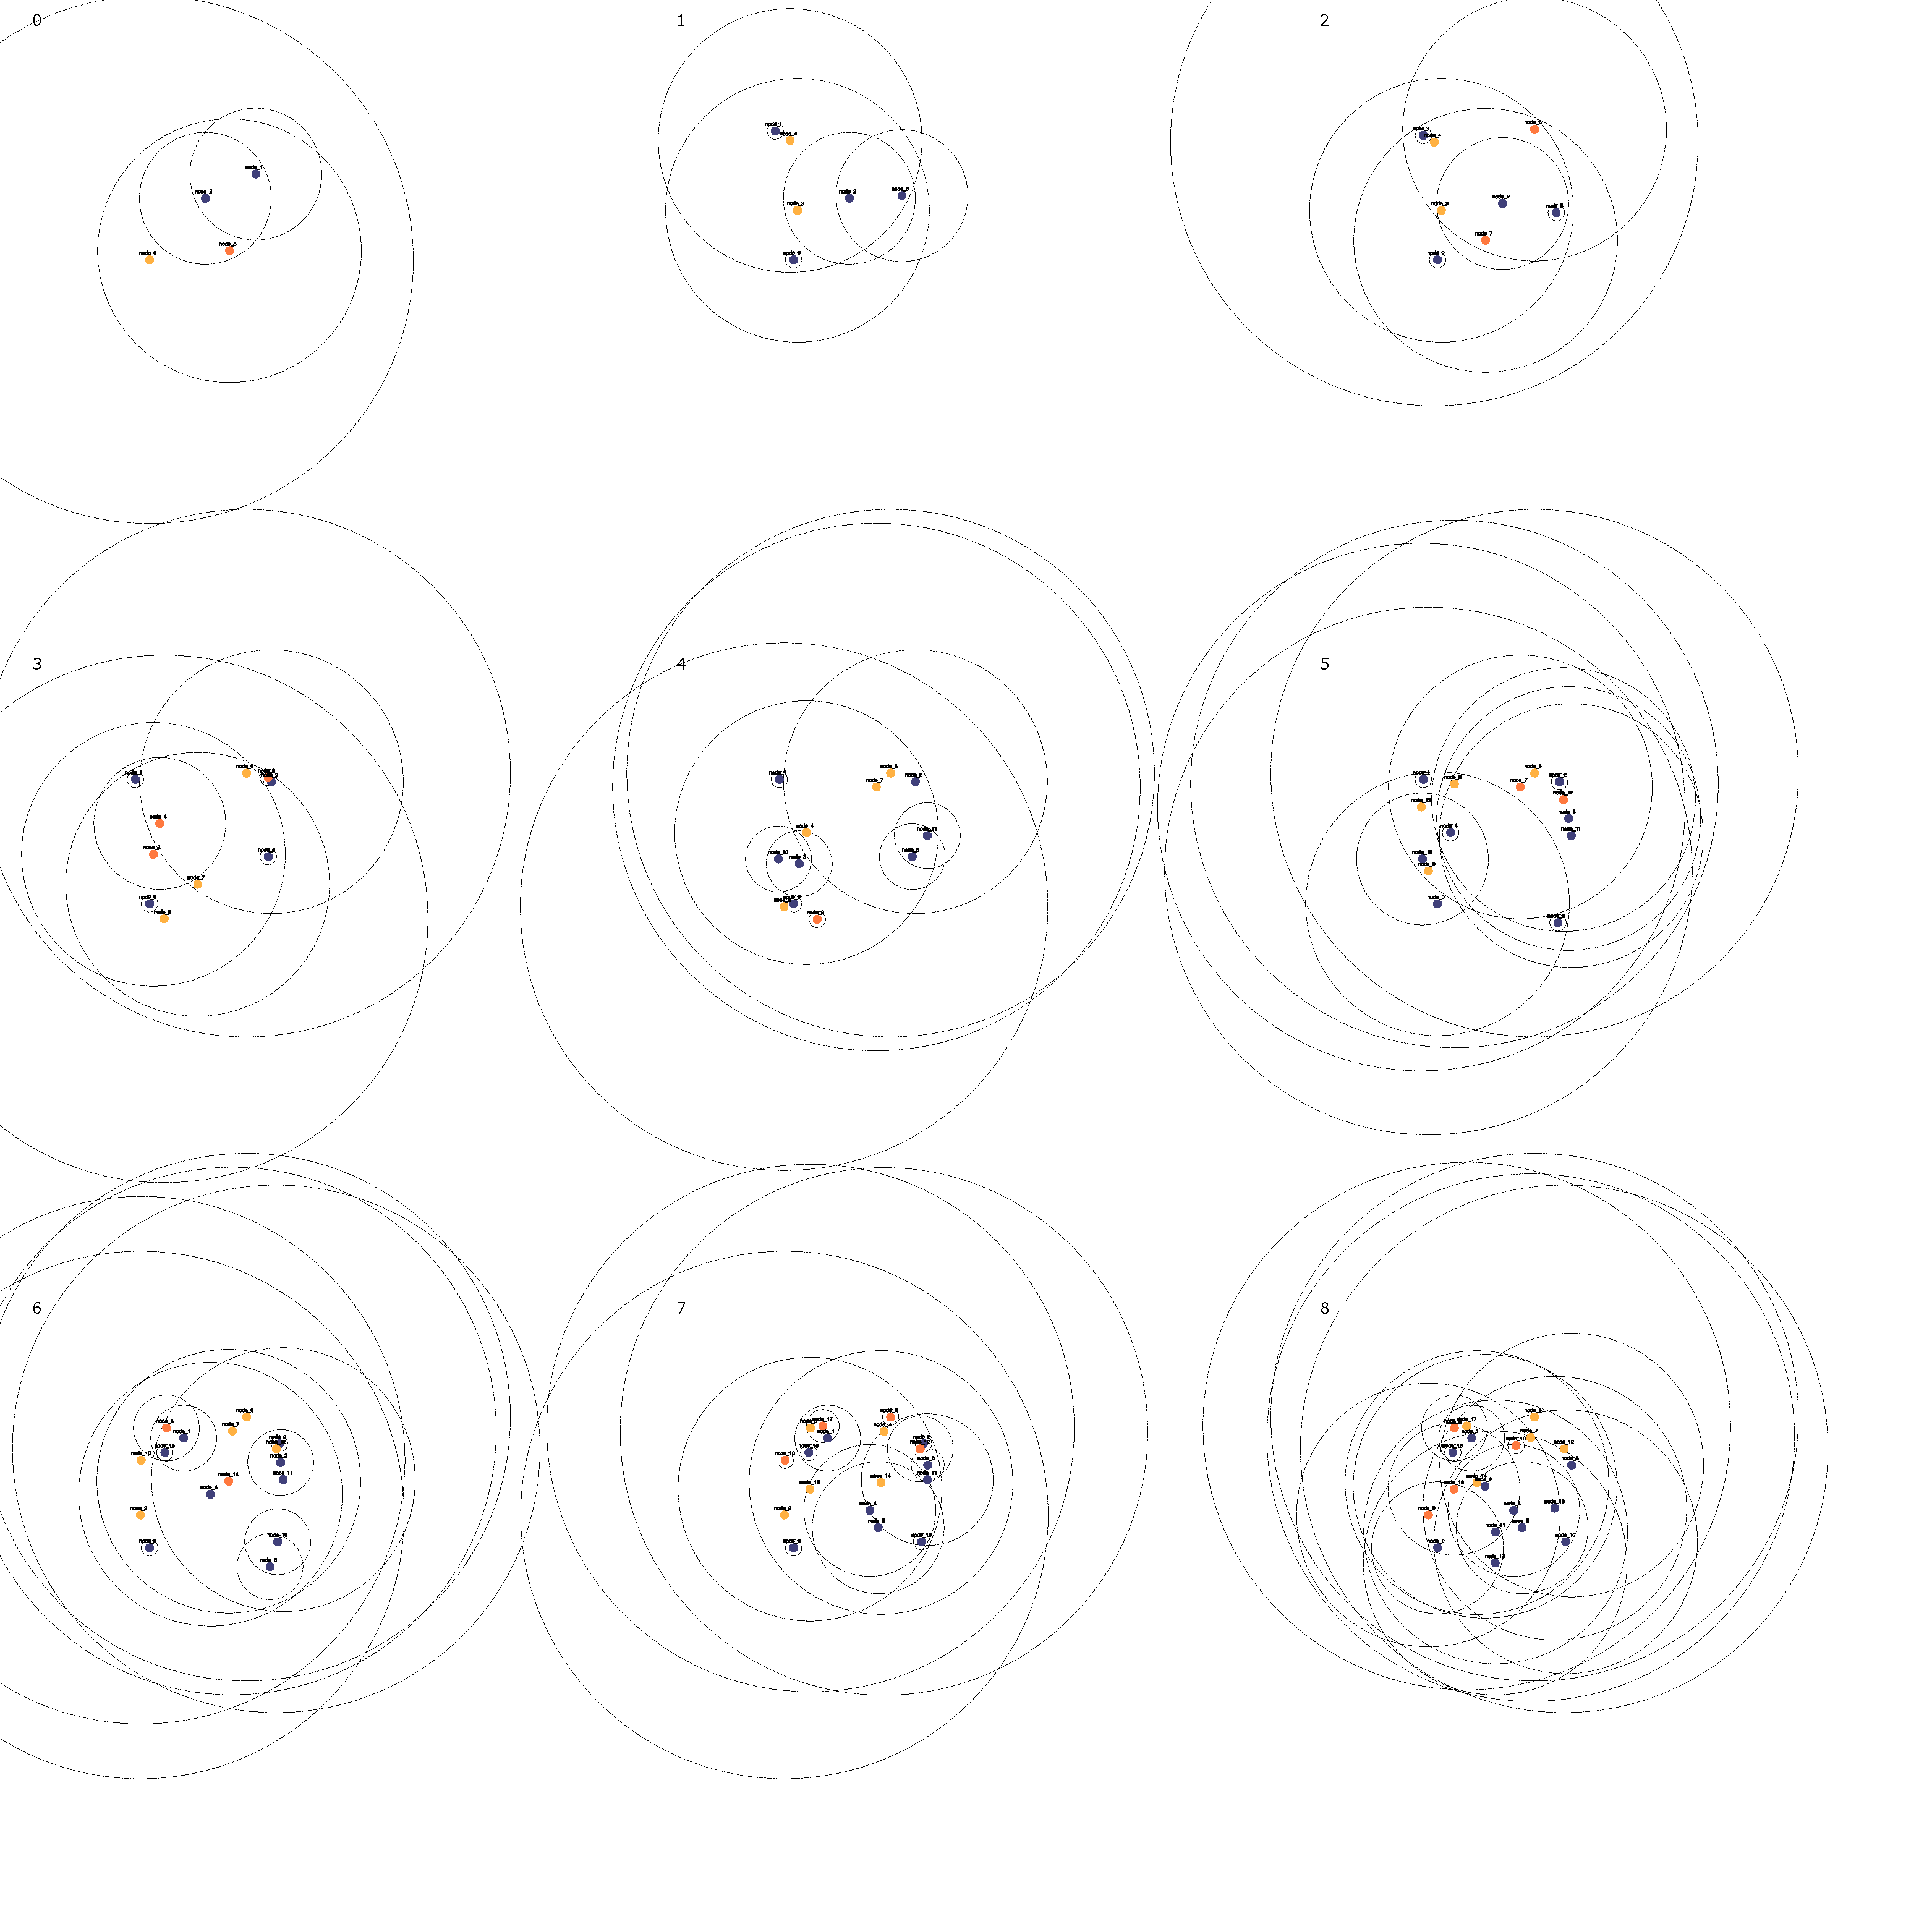
\includegraphics[width=350pt]{figures/LocarnoTreaties-RandomFinal}
\caption{Graphs of the system using random lottery at each epoch, the levels
    are depicted in different colors.} \label{fig:LocarnoTreaties-RandomFinal}
\end{figure}

\begin{figure}[!h] 
\centering
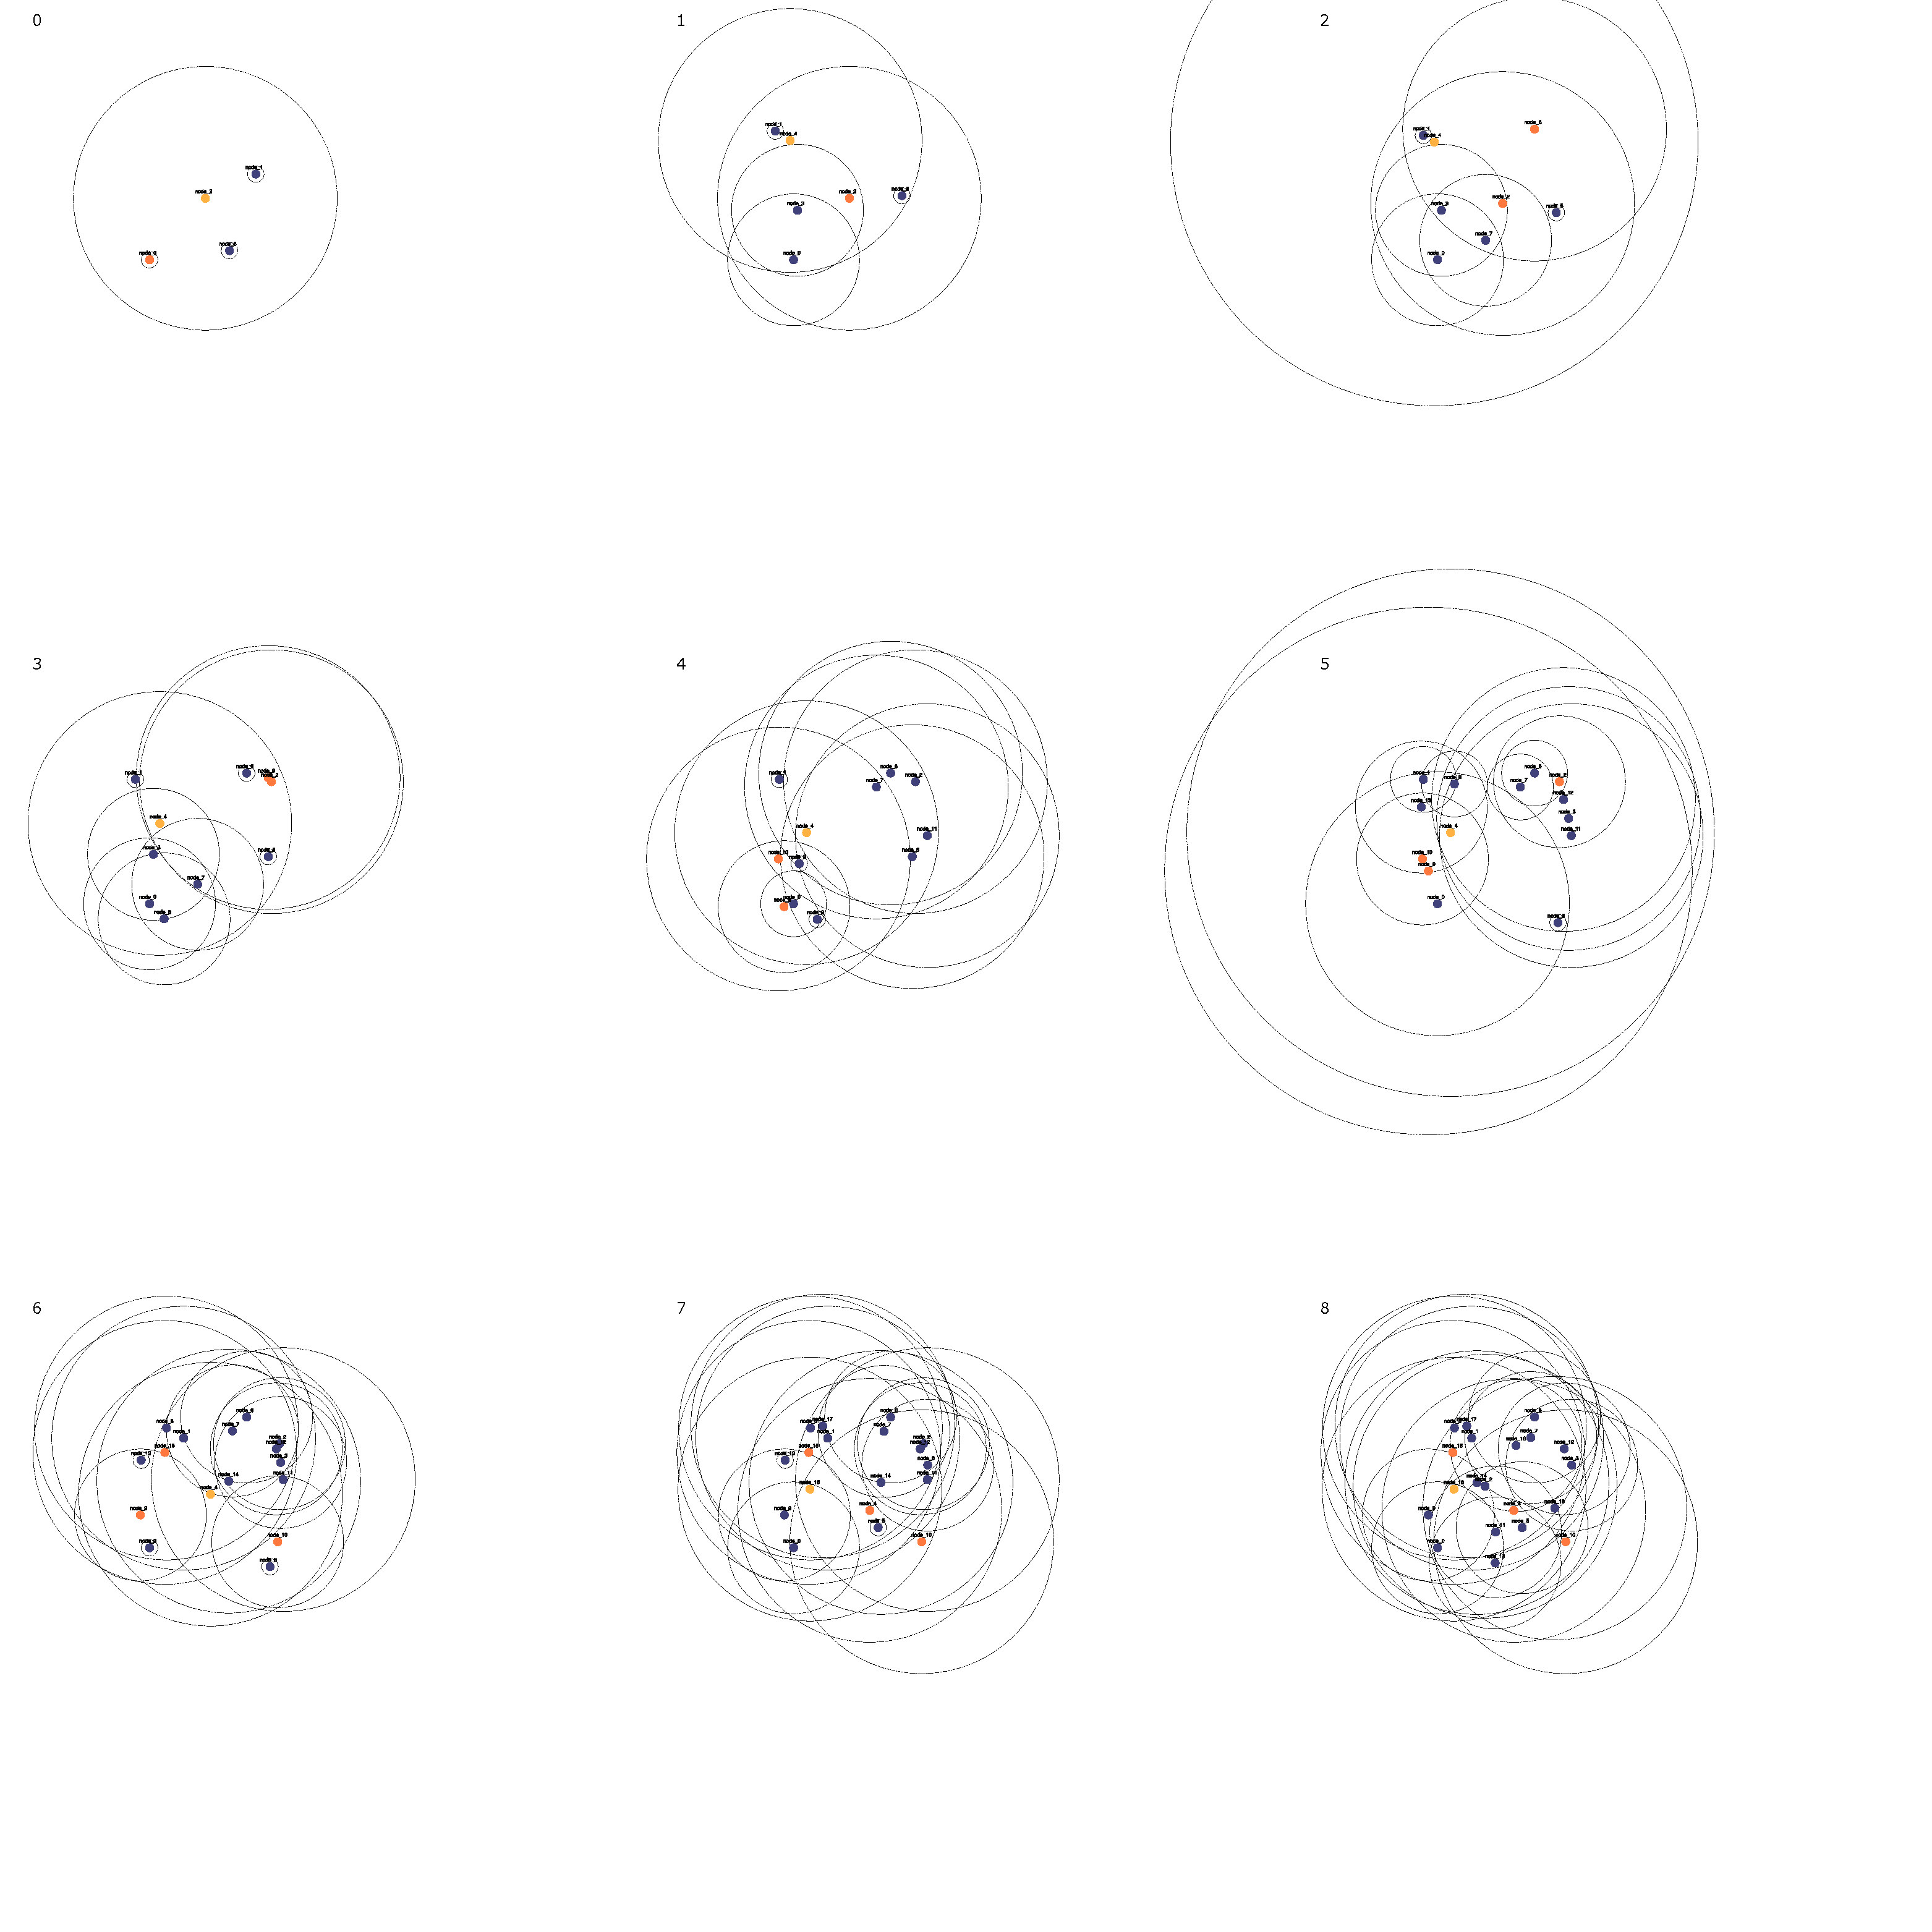
\includegraphics[width=500pt]{figures/LocarnoTreaties-LocarnoFinal}
\caption{Graphs of the system using \textit{Locarno Treaties} lottery at each
  epoch, the levels are depicted in different colors.}
  \label{fig:LocarnoTreaties-LocarnoFinal}
\end{figure}

\chapter{Space Time : Data} \label{app:SpaceTime-data}

\begin{figure}[!h] 
\centering
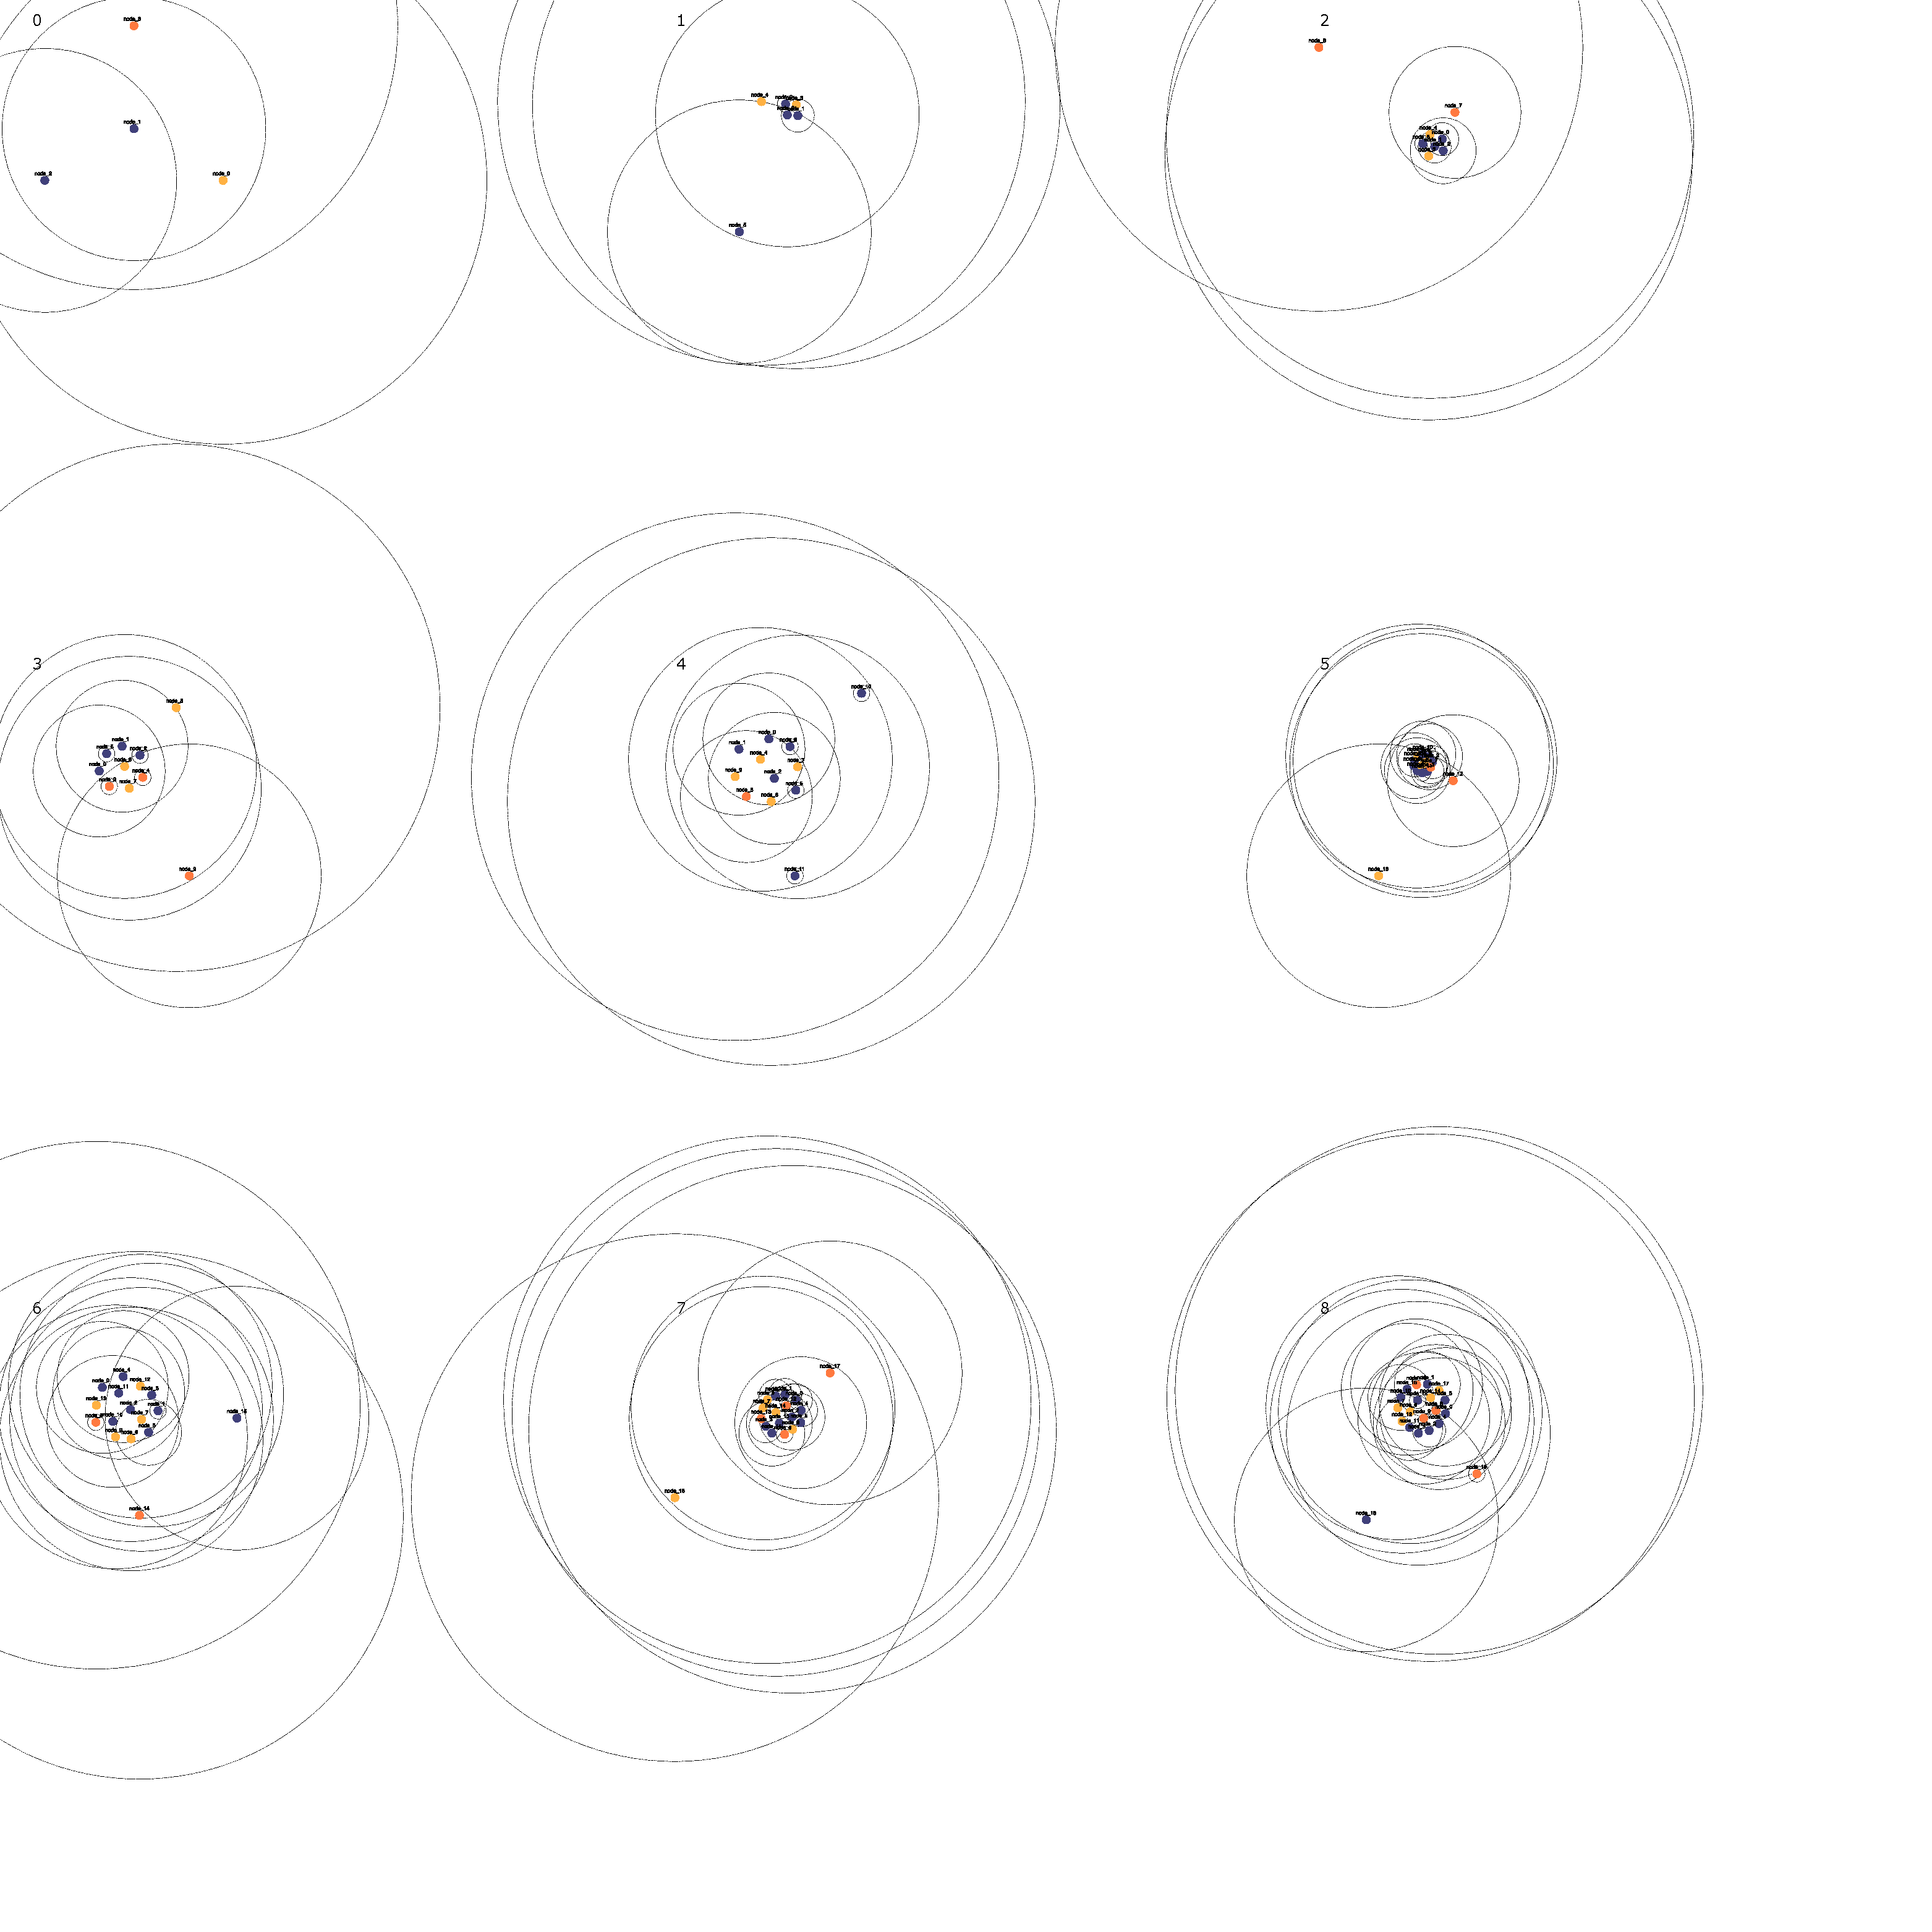
\includegraphics[width=350pt]{figures/SpaceTime-Random}
\caption{Graphs of the system using the new definition of the distance and
    random lottery at each epoch, the levels are depicted in different colors.}
    \label{fig:SpaceTime-Random}
\end{figure}

\begin{figure}[!h] 
\centering
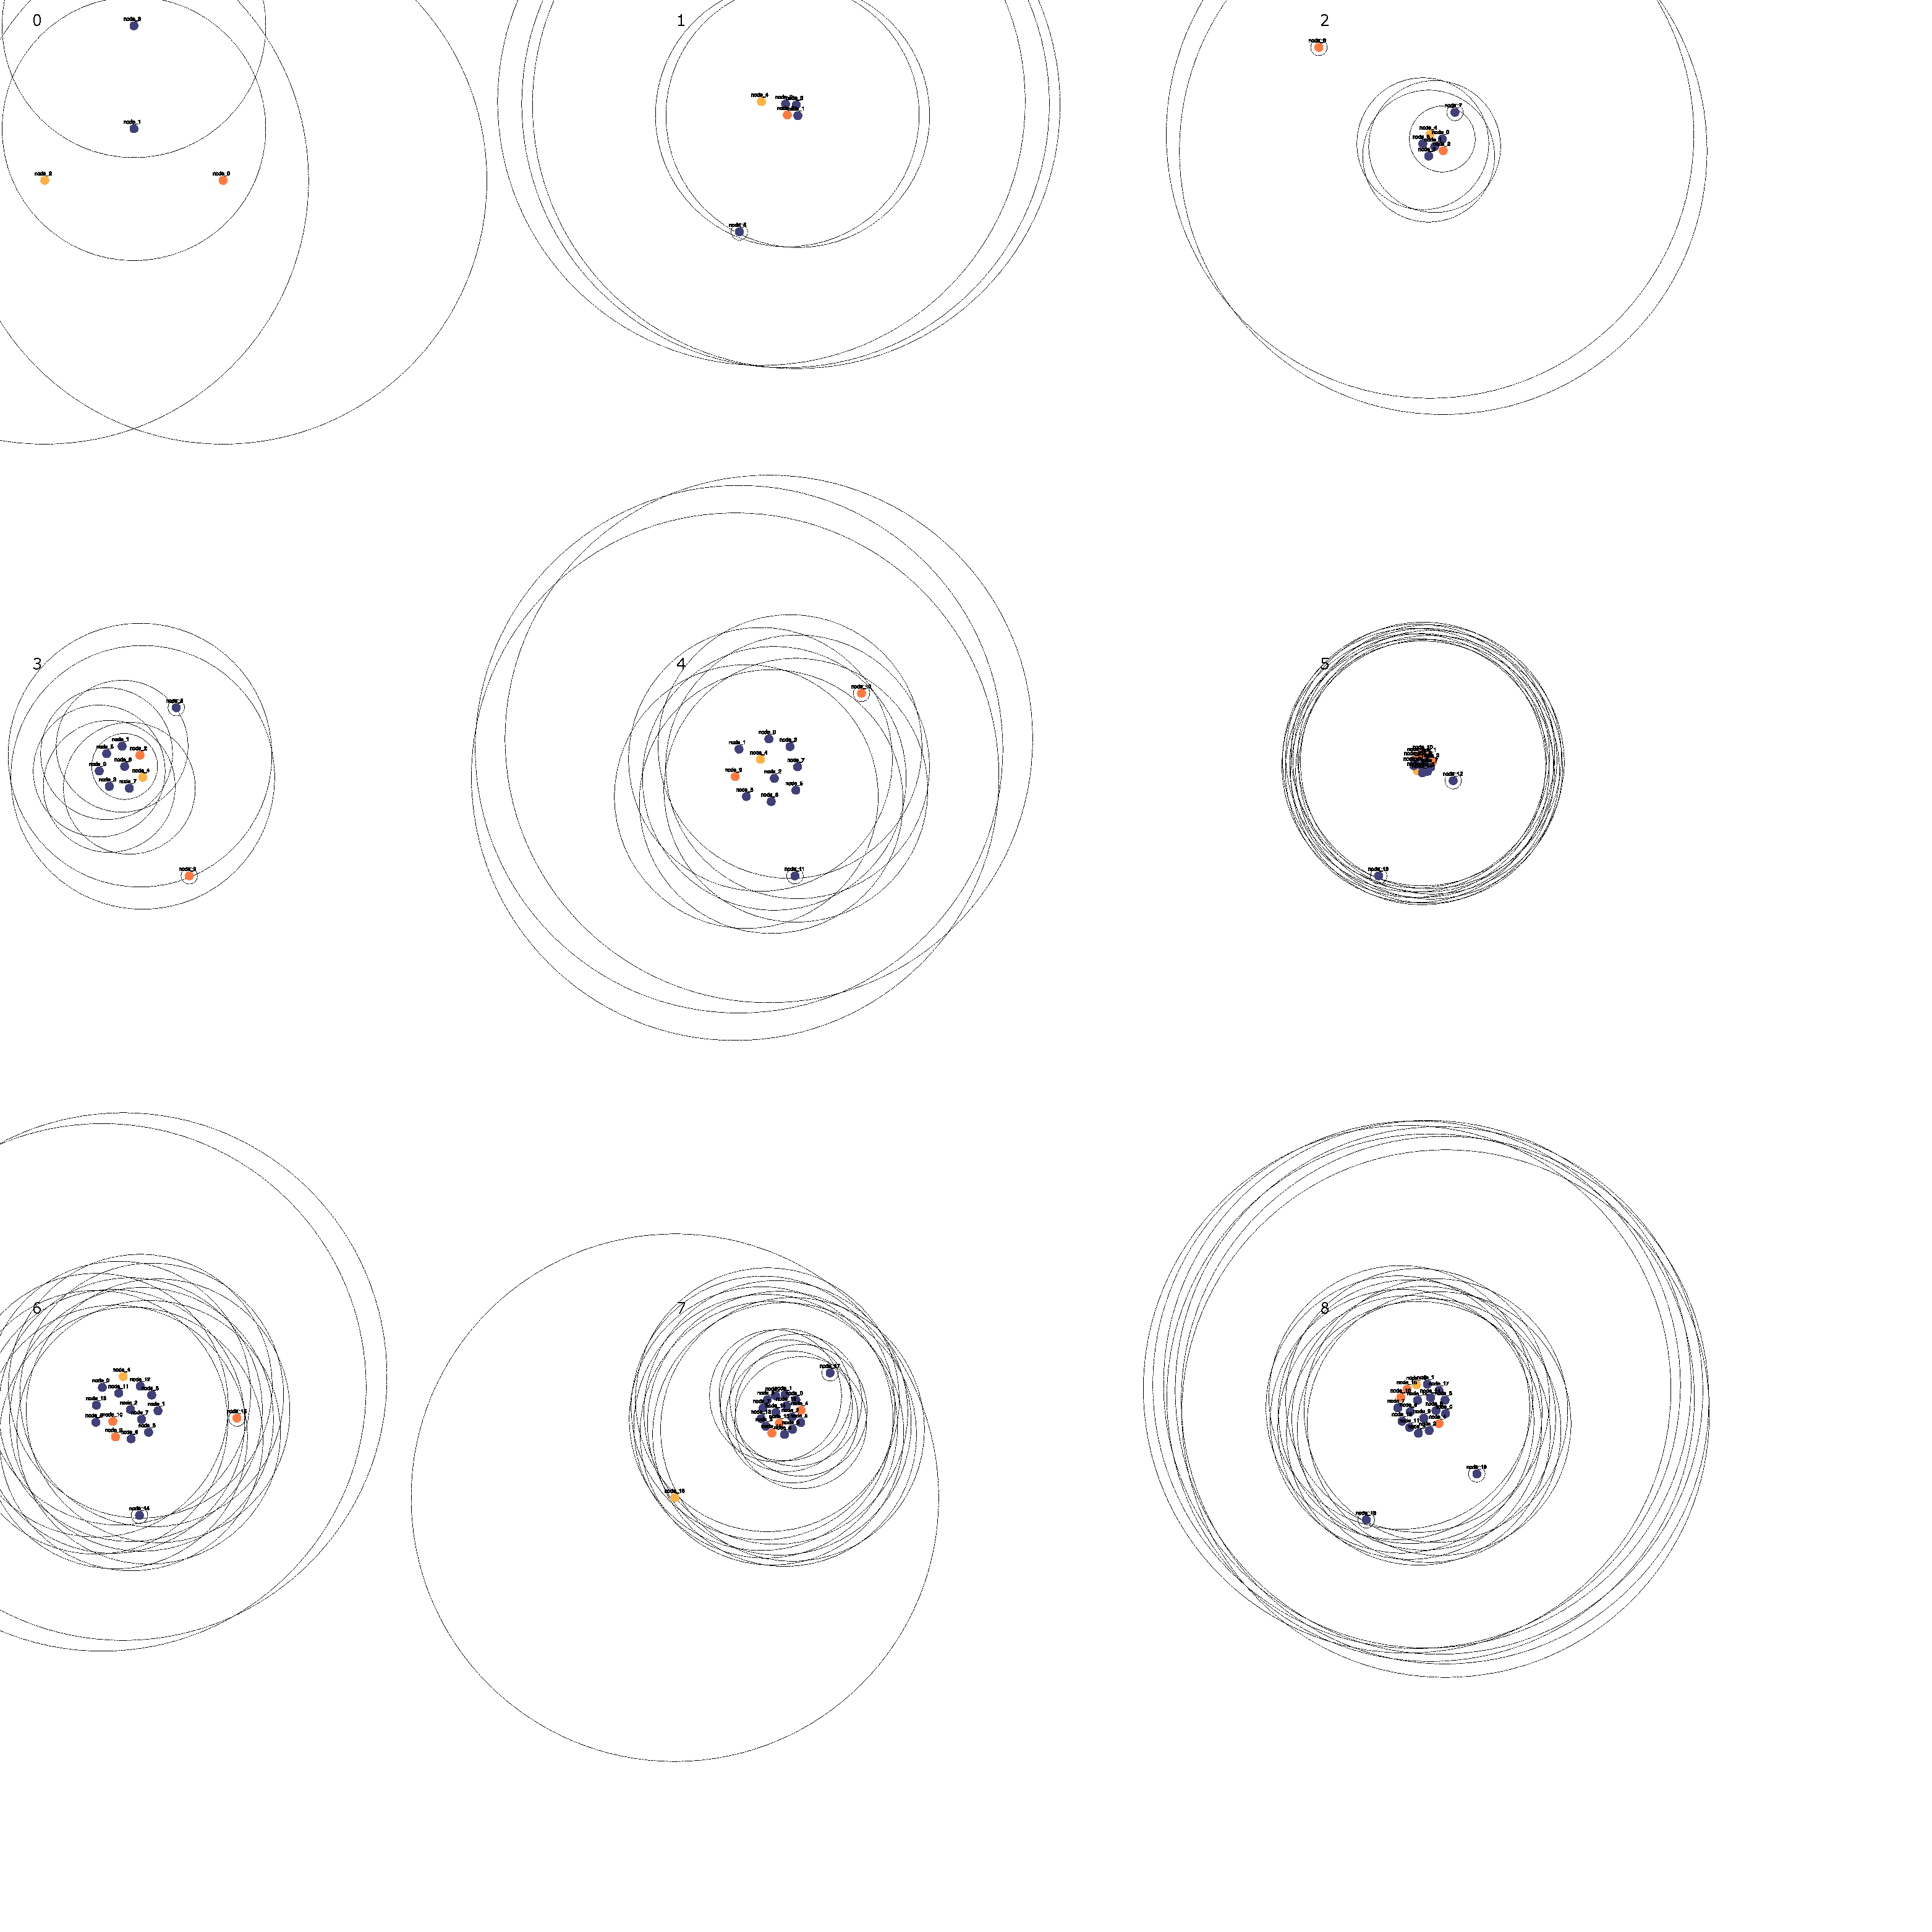
\includegraphics[width=500pt]{figures/SpaceTime-Locarno}
\caption{Graphs of the system using the new definition of the distance and
    \textit{Locarno Treaties} lottery at each epoch, the levels are depicted in
    different colors.} \label{fig:SpaceTime-Locarno}
\end{figure}

\begin{table}[h]
\centering
\tiny
\begin{tabular}{@{}llrrrrrrll@{}}
\toprule
& \textbf{Name}   &\textbf{Random Level} &\textbf{Locarno Level} & \textbf{X} & \textbf{Y} & \textbf{SpaceTime X} & \textbf{SpaceTime Y}  \\ \midrule
\textbf{0} & Node 0&$0$&$0$&$40.31$&$254.23$&$24.79$&$-48.22$&\\ \hdashline
\textbf{1} & Node 1&$0$&$0$&$60.26$&$98.32$&$48.49$&$-25.58$&\\ \hdashline
\textbf{2} & Node 2&$0$&$1$&$148.63$&$134.85$&$28.17$&$-26.93$&\\ \hdashline
\textbf{3} & Node 3&$2$&$0$&$195.48$&$236.62$&$45.51$&$-46.47$&\\ \hdashline
\textbf{4} & Node 4&$2$&$2$&$31.55$&$26.72$&$-22.07$&$-52.79$&\\ \hdashline
\textbf{5} & Node 5&$0$&$0$&$250.73$&$129.83$&$-64.90$&$200.00$&\\ \hdashline\midrule
\bottomrule
\end{tabular}
\caption{Description of the system for Epoch 1.}
\end{table}

\begin{table}[h]
\centering
\tiny
\begin{tabular}{@{}llrrrrrrll@{}}
\toprule
& \textbf{Name}   &\textbf{Random Level} &\textbf{Locarno Level} & \textbf{X} & \textbf{Y} & \textbf{SpaceTime X} & \textbf{SpaceTime Y}  \\ \midrule
\textbf{0} & Node 0&$0$&$0$&$40.31$&$254.23$&$49.46$&$19.91$&\\ \hdashline
\textbf{1} & Node 1&$0$&$0$&$21.96$&$259.85$&$34.73$&$34.54$&\\ \hdashline
\textbf{2} & Node 2&$0$&$1$&$148.63$&$134.85$&$51.27$&$42.54$&\\ \hdashline
\textbf{3} & Node 3&$2$&$0$&$201.12$&$27.50$&$23.04$&$53.01$&\\ \hdashline
\textbf{4} & Node 4&$2$&$2$&$49.25$&$27.52$&$25.75$&$11.01$&\\ \hdashline
\textbf{5} & Node 5&$0$&$0$&$250.73$&$129.83$&$11.69$&$28.96$&\\ \hdashline
\textbf{6} & Node 6&$1$&$1$&$237.37$&$23.28$&$-190.00$&$-158.04$&\\ \hdashline
\textbf{7} & Node 7&$1$&$0$&$151.83$&$224.03$&$74.06$&$-31.92$&\\ \hdashline\midrule
\bottomrule
\end{tabular}
\caption{Description of the system for Epoch 2.}
\end{table}

\begin{table}[h]
\centering
\tiny
\begin{tabular}{@{}llrrrrrrll@{}}
\toprule
& \textbf{Name}   &\textbf{Random Level} &\textbf{Locarno Level} & \textbf{X} & \textbf{Y} & \textbf{SpaceTime X} & \textbf{SpaceTime Y}  \\ \midrule
\textbf{0} & Node 0&$0$&$0$&$40.31$&$254.23$&$-57.44$&$-3.48$&\\ \hdashline
\textbf{1} & Node 1&$0$&$0$&$21.96$&$259.85$&$-12.92$&$-51.60$&\\ \hdashline
\textbf{2} & Node 2&$0$&$1$&$148.63$&$134.85$&$21.74$&$-34.24$&\\ \hdashline
\textbf{3} & Node 3&$1$&$0$&$294.78$&$88.66$&$-37.94$&$26.42$&\\ \hdashline
\textbf{4} & Node 4&$1$&$2$&$54.87$&$47.19$&$27.06$&$8.88$&\\ \hdashline
\textbf{5} & Node 5&$0$&$0$&$274.02$&$290.94$&$-43.06$&$-37.13$&\\ \hdashline
\textbf{6} & Node 6&$2$&$0$&$237.37$&$23.28$&$-8.13$&$-12.40$&\\ \hdashline
\textbf{7} & Node 7&$2$&$0$&$151.83$&$224.03$&$1.12$&$30.00$&\\ \hdashline
\textbf{8} & Node 8&$2$&$0$&$68.63$&$283.58$&$92.18$&$-126.46$&\\ \hdashline
\textbf{9} & Node 9&$1$&$1$&$270.43$&$9.18$&$117.42$&$200.00$&\\ \hdashline\midrule
\bottomrule
\end{tabular}
\caption{Description of the system for Epoch 3.}
\end{table}

\begin{table}[h]
\centering
\tiny
\begin{tabular}{@{}llrrrrrrll@{}}
\toprule
& \textbf{Name}   &\textbf{Random Level} &\textbf{Locarno Level} & \textbf{X} & \textbf{Y} & \textbf{SpaceTime X} & \textbf{SpaceTime Y}  \\ \midrule
\textbf{0} & Node 0&$0$&$0$&$40.31$&$254.23$&$-7.61$&$-65.71$&\\ \hdashline
\textbf{1} & Node 1&$0$&$0$&$21.96$&$259.85$&$-65.57$&$-45.77$&\\ \hdashline
\textbf{2} & Node 2&$0$&$0$&$94.82$&$270.93$&$2.92$&$10.83$&\\ \hdashline
\textbf{3} & Node 3&$0$&$0$&$73.13$&$21.70$&$33.37$&$-50.91$&\\ \hdashline
\textbf{4} & Node 4&$2$&$2$&$22.54$&$190.61$&$-23.89$&$-26.00$&\\ \hdashline
\textbf{5} & Node 5&$0$&$0$&$274.02$&$290.94$&$44.76$&$33.88$&\\ \hdashline
\textbf{6} & Node 6&$2$&$0$&$237.37$&$23.28$&$-3.04$&$55.86$&\\ \hdashline
\textbf{7} & Node 7&$2$&$0$&$284.77$&$51.97$&$48.17$&$-11.59$&\\ \hdashline
\textbf{8} & Node 8&$1$&$0$&$289.02$&$242.48$&$-51.31$&$46.13$&\\ \hdashline
\textbf{9} & Node 9&$2$&$1$&$270.43$&$9.18$&$-73.01$&$7.58$&\\ \hdashline
\textbf{10} & Node 10&$0$&$1$&$17.92$&$180.81$&$172.23$&$-154.31$&\\ \hdashline
\textbf{11} & Node 11&$0$&$0$&$281.74$&$114.36$&$43.01$&$200.00$&\\ \hdashline\midrule
\bottomrule
\end{tabular}
\caption{Description of the system for Epoch 4.}
\end{table}

\begin{table}[h]
\centering
\tiny
\begin{tabular}{@{}llrrrrrrll@{}}
\toprule
& \textbf{Name}   &\textbf{Random Level} &\textbf{Locarno Level} & \textbf{X} & \textbf{Y} & \textbf{SpaceTime X} & \textbf{SpaceTime Y}  \\ \midrule
\textbf{0} & Node 0&$0$&$0$&$40.31$&$254.23$&$-4.61$&$-24.37$&\\ \hdashline
\textbf{1} & Node 1&$0$&$0$&$195.36$&$135.24$&$24.83$&$-31.13$&\\ \hdashline
\textbf{2} & Node 2&$0$&$1$&$121.80$&$59.15$&$30.13$&$-20.63$&\\ \hdashline
\textbf{3} & Node 3&$0$&$0$&$78.31$&$38.28$&$21.02$&$-2.93$&\\ \hdashline
\textbf{4} & Node 4&$0$&$2$&$22.54$&$190.61$&$0.92$&$-4.09$&\\ \hdashline
\textbf{5} & Node 5&$0$&$0$&$158.61$&$150.27$&$-5.84$&$-13.89$&\\ \hdashline
\textbf{6} & Node 6&$2$&$0$&$237.37$&$23.28$&$9.32$&$-14.03$&\\ \hdashline
\textbf{7} & Node 7&$1$&$0$&$284.77$&$51.97$&$27.10$&$-10.89$&\\ \hdashline
\textbf{8} & Node 8&$2$&$0$&$294.03$&$246.83$&$15.94$&$-24.40$&\\ \hdashline
\textbf{9} & Node 9&$2$&$1$&$204.49$&$215.15$&$1.63$&$-32.49$&\\ \hdashline
\textbf{10} & Node 10&$0$&$1$&$17.92$&$180.81$&$11.97$&$-36.47$&\\ \hdashline
\textbf{11} & Node 11&$0$&$0$&$296.34$&$115.18$&$10.98$&$0.09$&\\ \hdashline
\textbf{12} & Node 12&$1$&$0$&$64.98$&$126.63$&$70.62$&$15.25$&\\ \hdashline
\textbf{13} & Node 13&$2$&$0$&$8.71$&$66.51$&$-74.01$&$200.00$&\\ \hdashline\midrule
\bottomrule
\end{tabular}
\caption{Description of the system for Epoch 5.}
\end{table}

\begin{table}[h]
\centering
\tiny
\begin{tabular}{@{}llrrrrrrll@{}}
\toprule
& \textbf{Name}   &\textbf{Random Level} &\textbf{Locarno Level} & \textbf{X} & \textbf{Y} & \textbf{SpaceTime X} & \textbf{SpaceTime Y}  \\ \midrule
\textbf{0} & Node 0&$0$&$0$&$40.31$&$254.23$&$-51.31$&$-57.07$&\\ \hdashline
\textbf{1} & Node 1&$0$&$0$&$195.36$&$135.24$&$56.70$&$-11.64$&\\ \hdashline
\textbf{2} & Node 2&$0$&$0$&$121.80$&$59.15$&$3.24$&$-13.90$&\\ \hdashline
\textbf{3} & Node 3&$0$&$0$&$78.31$&$38.28$&$44.51$&$-42.24$&\\ \hdashline
\textbf{4} & Node 4&$0$&$2$&$22.54$&$190.61$&$-10.86$&$-78.06$&\\ \hdashline
\textbf{5} & Node 5&$0$&$0$&$158.61$&$150.27$&$38.49$&$30.07$&\\ \hdashline
\textbf{6} & Node 6&$2$&$0$&$237.37$&$23.28$&$4.57$&$42.91$&\\ \hdashline
\textbf{7} & Node 7&$2$&$0$&$307.43$&$56.86$&$24.73$&$4.95$&\\ \hdashline
\textbf{8} & Node 8&$1$&$0$&$294.03$&$246.83$&$-63.98$&$10.68$&\\ \hdashline
\textbf{9} & Node 9&$2$&$1$&$204.49$&$215.15$&$-25.86$&$39.11$&\\ \hdashline
\textbf{10} & Node 10&$0$&$1$&$33.84$&$197.23$&$-30.96$&$9.05$&\\ \hdashline
\textbf{11} & Node 11&$0$&$0$&$188.26$&$181.69$&$-19.49$&$-45.90$&\\ \hdashline
\textbf{12} & Node 12&$2$&$0$&$132.69$&$134.87$&$22.46$&$-59.31$&\\ \hdashline
\textbf{13} & Node 13&$2$&$0$&$8.71$&$66.51$&$-62.99$&$-22.44$&\\ \hdashline
\textbf{14} & Node 14&$1$&$0$&$131.37$&$148.74$&$20.75$&$191.27$&\\ \hdashline
\textbf{15} & Node 15&$0$&$1$&$69.93$&$69.26$&$210.00$&$2.51$&\\ \hdashline\midrule
\bottomrule
\end{tabular}
\caption{Description of the system for Epoch 6.}
\end{table}

\begin{table}[h]
\centering
\tiny
\begin{tabular}{@{}llrrrrrrll@{}}
\toprule
& \textbf{Name}   &\textbf{Random Level} &\textbf{Locarno Level} & \textbf{X} & \textbf{Y} & \textbf{SpaceTime X} & \textbf{SpaceTime Y}  \\ \midrule
\textbf{0} & Node 0&$0$&$0$&$40.31$&$254.23$&$44.82$&$-32.46$&\\ \hdashline
\textbf{1} & Node 1&$0$&$0$&$195.36$&$135.24$&$23.69$&$-42.40$&\\ \hdashline
\textbf{2} & Node 2&$0$&$0$&$127.36$&$71.11$&$37.25$&$0.45$&\\ \hdashline
\textbf{3} & Node 3&$0$&$0$&$78.31$&$38.28$&$-13.90$&$18.27$&\\ \hdashline
\textbf{4} & Node 4&$0$&$1$&$22.54$&$190.61$&$54.95$&$-12.59$&\\ \hdashline
\textbf{5} & Node 5&$0$&$0$&$158.61$&$150.27$&$54.23$&$11.40$&\\ \hdashline
\textbf{6} & Node 6&$1$&$0$&$237.37$&$23.28$&$22.88$&$34.34$&\\ \hdashline
\textbf{7} & Node 7&$2$&$0$&$307.43$&$56.86$&$-18.81$&$-17.10$&\\ \hdashline
\textbf{8} & Node 8&$2$&$0$&$153.08$&$223.42$&$38.19$&$24.37$&\\ \hdashline
\textbf{9} & Node 9&$2$&$0$&$116.75$&$127.76$&$-10.41$&$-33.05$&\\ \hdashline
\textbf{10} & Node 10&$0$&$1$&$152.15$&$283.84$&$12.76$&$12.53$&\\ \hdashline
\textbf{11} & Node 11&$0$&$0$&$188.26$&$181.69$&$5.31$&$-40.87$&\\ \hdashline
\textbf{12} & Node 12&$1$&$0$&$132.69$&$134.87$&$26.25$&$-21.53$&\\ \hdashline
\textbf{13} & Node 13&$1$&$0$&$8.71$&$66.51$&$-22.57$&$3.59$&\\ \hdashline
\textbf{14} & Node 14&$2$&$0$&$131.37$&$148.74$&$5.87$&$-8.45$&\\ \hdashline
\textbf{15} & Node 15&$0$&$1$&$86.54$&$79.72$&$-1.75$&$31.73$&\\ \hdashline
\textbf{16} & Node 16&$2$&$2$&$65.63$&$137.88$&$-190.00$&$157.01$&\\ \hdashline
\textbf{17} & Node 17&$1$&$0$&$100.00$&$20.72$&$111.23$&$-85.22$&\\ \hdashline\midrule
\bottomrule
\end{tabular}
\caption{Description of the system for Epoch 7.}
\end{table}


\begin{table}[h]
\centering
\tiny
\begin{tabular}{@{}llrrrrrrll@{}}
\toprule
& \textbf{Name}   &\textbf{Random Level} &\textbf{Locarno Level} & \textbf{X} & \textbf{Y} & \textbf{SpaceTime X} & \textbf{SpaceTime Y}  \\ \midrule
\textbf{0} & Node 0&$0$&$0$&$40.31$&$254.23$&$55.84$&$-6.18$&\\ \hdashline
\textbf{1} & Node 1&$0$&$0$&$211.18$&$244.47$&$20.42$&$-63.24$&\\ \hdashline
\textbf{2} & Node 2&$0$&$0$&$127.36$&$71.11$&$23.97$&$26.69$&\\ \hdashline
\textbf{3} & Node 3&$0$&$0$&$94.11$&$55.61$&$3.17$&$32.03$&\\ \hdashline
\textbf{4} & Node 4&$0$&$1$&$36.39$&$192.52$&$43.25$&$13.27$&\\ \hdashline
\textbf{5} & Node 5&$0$&$0$&$158.61$&$150.27$&$54.84$&$-32.35$&\\ \hdashline
\textbf{6} & Node 6&$2$&$0$&$259.99$&$52.13$&$-12.69$&$-10.00$&\\ \hdashline
\textbf{7} & Node 7&$2$&$0$&$307.43$&$56.86$&$-36.79$&$-17.48$&\\ \hdashline
\textbf{8} & Node 8&$1$&$0$&$153.08$&$223.42$&$37.13$&$-12.09$&\\ \hdashline
\textbf{9} & Node 9&$1$&$0$&$116.75$&$127.76$&$13.46$&$2.65$&\\ \hdashline
\textbf{10} & Node 10&$0$&$1$&$239.23$&$257.28$&$-31.06$&$-37.56$&\\ \hdashline
\textbf{11} & Node 11&$0$&$0$&$188.26$&$181.69$&$-13.74$&$20.71$&\\ \hdashline
\textbf{12} & Node 12&$2$&$0$&$132.69$&$134.87$&$-28.60$&$8.46$&\\ \hdashline
\textbf{13} & Node 13&$0$&$0$&$8.71$&$66.51$&$1.51$&$-31.86$&\\ \hdashline
\textbf{14} & Node 14&$2$&$0$&$145.68$&$155.97$&$26.88$&$-37.18$&\\ \hdashline
\textbf{15} & Node 15&$0$&$1$&$43.55$&$199.44$&$-18.76$&$-53.44$&\\ \hdashline
\textbf{16} & Node 16&$1$&$2$&$73.22$&$140.48$&$-0.38$&$-62.24$&\\ \hdashline
\textbf{17} & Node 17&$2$&$0$&$56.03$&$16.60$&$43.18$&$-51.05$&\\ \hdashline
\textbf{18} & Node 18&$0$&$0$&$82.08$&$35.23$&$-98.10$&$200.00$&\\ \hdashline
\textbf{19} & Node 19&$1$&$0$&$193.24$&$68.52$&$116.45$&$110.87$&\\ \hdashline\midrule
\bottomrule
\end{tabular}
\caption{Description of the system for Epoch 8.}
\end{table}

\chapter{Dataset on Master Thesis}
Here are some important random facts about this master's thesis. The
aggregation of data was stopped the day of the printing. 
\begin{table}[h]
\centering
\begin{tabular}{@{}lrrrr@{}}
\toprule
\textbf{Language}   &\textbf{Files} & \textbf{Blank} & \textbf{Comment} & \textbf{Code} \\ \midrule
Go    & 26 & 1'272 & 841  & 4'285 \\ \hdashline
TeX    & 8  & 316 & 124  & 2'061 \\ \hdashline
Jupyter Notebook & 4  & 0  & 2312  & 449 \\ \hdashline
Python   & 4  & 79 & 2  & 315 \\ \hdashline
Markdown   & 4  & 60 & 0  & 135 \\ \midrule
Total   & 47 & 1'732 & 3'279 & 7'241 \\
\midrule
\bottomrule
\end{tabular}
\caption{Line of code for the different languages used in that project.}
\label{tab:my-table}
\end{table}

\begin{table}[h]
\centering
\begin{tabular}{@{}lr@{}}
\toprule
\textbf{Number of}    & \textbf{Total} \\ \midrule
 Commits & 192 \\ \hdashline
 Coffees & 276 \\ \hdashline
Days & 90 \\ \hdashline
Graphs & 28 \\
\midrule
\bottomrule
\end{tabular}
\caption{Some random stats.}
\label{tab:my-table}
\end{table}


\end{document}
